% !TEX root = ./LECTURE.tex
%--------------------------------------------------------------------------------
\chapter{線形システム論（連続時間系） \label{sec_cont_sys}}
%---------------------------------------------------------------------------

本章では線形システム理論（状態方程式であらわされたシステムに対する制御理論）に基づいて制御系を設計する方法について説明する．ここでは理論を応用する立場にたち，直感的な議論を中心とし，厳密な定義や証明は最低限しか行っていない．理論を展開・発展させるために重要な数学的定義や証明については成書を参照されたい．

なお，本資料では，読者が伝達関数を用いた制御理論に対する知識を持っていることを仮定するが，これらを知らない場合にも，関連個所を読み飛ばすことにより線形システム制御理論が理解できるように構成されている．

\section{状態方程式}
%---------------------------------------------------------------------------
Fig.\ref{fig:feedback}の制御対象（プラント）を考える．
ここでは，制御対象（プラント）を伝達関数$G(s)$により表現している．

\begin{figure}[htbp]
 \begin{center}
%  \input{figure/feedback.pstex} % scale = 1.0
  \input{figure/feedback.pstex_t} % scale = 1.0
  \caption{制御対象（プラント）}
  \label{fig:feedback}
 \end{center}
\end{figure}

これに対し，プラント$G(s)$の内部状態を表す変数$x$を新たに導入し，
プラント$G(s)$の入出力関係を1階の常微分方程式で表現したものが{\bf {状態方程式} (state equation)}であり，
一般に
\begin{align}
 \frac{dx}{dt} &= A x(t) + B u(t) \label{state_eq} \\
 y(t) &= C x(t) + D u(t) \label{output_eq}
\end{align}
のように表される．
ここで$x \in {\mathbb R}^n$, $ u \in {\mathbb R}^m $, $ y \in {\mathbb
R}^p $はそれぞれ{\bf {状態}(state)}，{\bf {入力}(input)}，{\bf {出力}(output)}である．

例えば力学においてよく用いられるFig.\ref{fig_mass}のようなバネ・
質量・ダンパー系の運動方程式も容易に状態方程式で表わされる．

\begin{figure}[h]
 \begin{center}
% \input{figure/spring-mass-damp.pstex_t} % scale = 90%
%　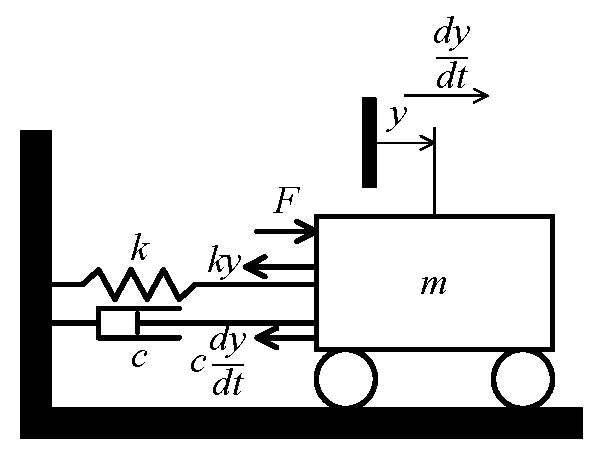
\epsfig{file=sfigure/car1.eps,scale=0.7}
	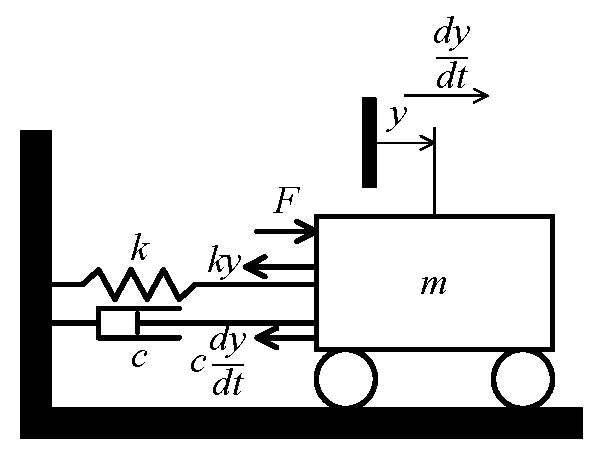
\includegraphics[width=0.4\linewidth]{sfigure/car1.eps}
  \caption{バネ・質量・ダンパー系}
  \label{fig_mass}
 \end{center}
\end{figure}

バネ定数を$k$, 質量を$m$, ダンパーの粘性係数を$c$, 質量の変位を$y$,
外力を$F$として，$m$に作用する力と加速度の関係を考えることで
バネ・質量・ダンパー系の運動方程式を表すと，
\begin{gather}
 m \frac{d^2y}{dt^2} + c \frac{dy}{dt} + k y = F
 \hspace*{1cm}
 (\mbox{または}m \frac{d^2y}{dt^2} = F - k y - c \frac{dy}{dt})
\end{gather}
となる．ここで，バネ・質量・ダンパー系のような機械系での定石として，
システムの状態を
\[
 \mbox{状態} = 
 \left(\begin{array}{c}
         \mbox{位置}\\
 	 \mbox{速度}
       \end{array}\right)
\]
と考える．すなわち，
\begin{gather}
 x = \left(\begin{array}{c}
            x_1 \\
	    x_2
	   \end{array}\right) 
 \defeq
 \left(\begin{array}{c}
         y \\
	\frac{dy}{dt}
       \end{array}\right)
\end{gather}
と定義すれば
\begin{align}
  \frac{dx_1}{dt} &= \frac{dy}{dt} \nonumber \\
                  &= x_2                     \\
  \frac{dx_2}{dt} &= \frac{d}{dt} \left\{\frac{dy}{dt} \right\} \nonumber \\
		  &= \frac{d^2 y}{dt^2} \nonumber \\
		  &= \frac{1}{m} (-c \frac{dy}{dt} -k y + F) \nonumber \\
		  &= -\frac{k}{m} x_1 - \frac{c}{m} x_2 + \frac{1}{m} F
\end{align}
であるから，これらをまとめて
\begin{align}
 \frac{d}{dt} \left(\begin{array}{c}
	             x_1 \\
		     x_2 
		    \end{array}\right)
 &=
 \left(\begin{array}{cc}
        0            &         1     \\
	-\frac{k}{m} & - \frac{c}{m} 
       \end{array}\right)
 \left(\begin{array}{c}
	x_1 \\
	x_2 
       \end{array}\right)
 +
 \left(\begin{array}{c}
        0 \\
	\frac{1}{m}
       \end{array}\right)
 F \label{eq:massstate} \\
 y &=
 \left(\begin{array}{cc}
             1 & 0 
       \end{array}\right)
 \left(\begin{array}{c}
        x_1 \\
	x_2 
       \end{array}\right) \label{eq:massoutput}
\end{align}
と状態方程式で表わされる．

制御対象を状態空間で表現する利点の一つとして，多入出力系も容易に扱うこと
ができることがある．例えば，Fig.\ref{fig:spring-2mass}のような，2質量系を考える．
2つの質量間のバネ定数を$k$, 質量をそれぞれ$m_1$, $m_2$, 
質量の平衡点からの変位をそれぞれ$y_1$, $y_2$,
外力をそれぞれ$F_1$, $F_2$として，運動方程式を表すと，
\begin{align}
 m_1 \frac{d^2y_1}{dt^2} - k (y_2 - y_1) &= F_1 \\
 m_2 \frac{d^2y_2}{dt^2} + k (y_2 - y_1) &= F_2
\end{align}
となる．ここで，バネ・質量・ダンパー系と同様の変形を行うことで，
2質量系の状態方程式を表すと，

\begin{figure}[t]
 \begin{center}
%  \input{figure/spring-2mass.pstex_t} % scale = 100%
　%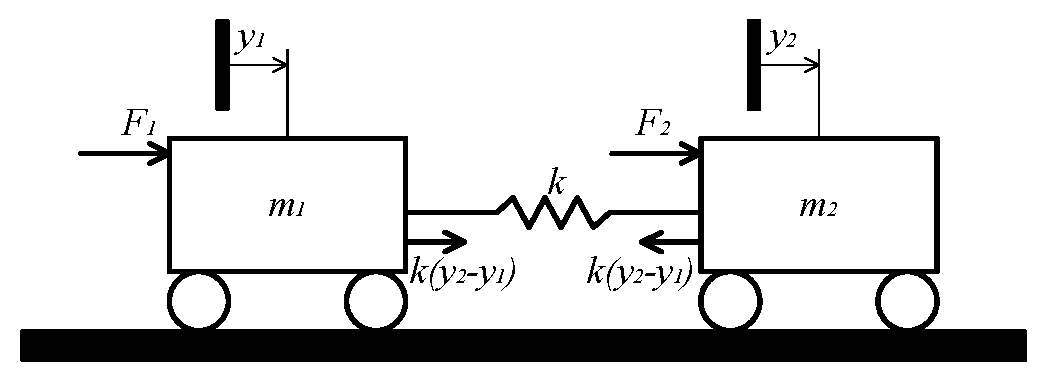
\epsfig{file=sfigure/car2.eps,scale=0.7}
	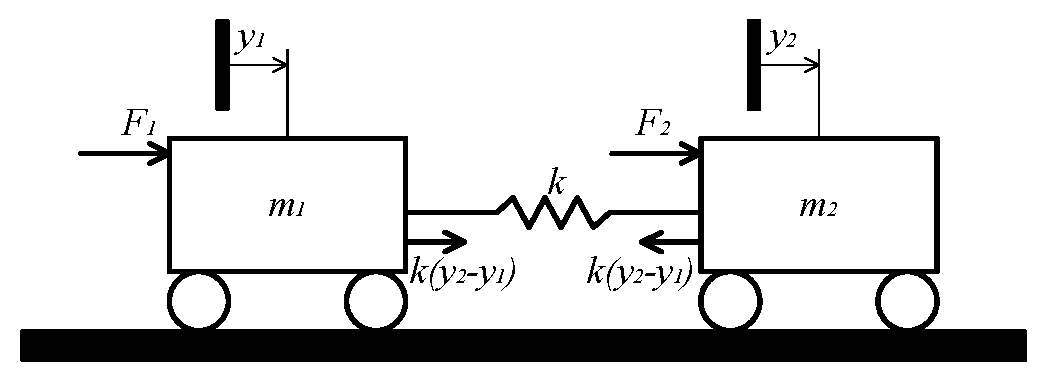
\includegraphics[width=0.7\linewidth]{sfigure/car2.eps}
  \caption{2質量系}
  \label{fig:spring-2mass}
 \end{center}
\end{figure}

\begin{align}
 \frac{d}{dt} \left(\begin{array}{c}
	             y_1 \\
		     y_2 \\
		     \frac{dy_1}{dt} \\
		     \frac{dy_2}{dt}
		    \end{array}\right)
 &=
 \left(\begin{array}{cccc}
        0 & 0 & 1 & 0     \\
        0 & 0 & 0 & 1     \\
	-\frac{k}{m_1} & \frac{k}{m_1} & 0 & 0 \\
	\frac{k}{m_2} & -\frac{k}{m_2} & 0 & 0 \\
       \end{array}\right)
 \left(\begin{array}{c}
        y_1 \\
	y_2 \\
	\frac{dy_1}{dt} \\
	\frac{dy_2}{dt}
       \end{array}\right)
 +
 \left(\begin{array}{cc}
        0 & 0 \\
        0 & 0 \\
	\frac{1}{m_1} & 0 \\
	0 & \frac{1}{m_2} \\
       \end{array}\right)
 \left(\begin{array}{c}
        F_1 \\
	F_2
       \end{array}\right) \\
 \left(\begin{array}{c}
        y_1 \\
	y_2
       \end{array}\right)
 &=
 \left(\begin{array}{cccc}
         1 & 0 & 0 & 0 \\
         0 & 1 & 0 & 0
       \end{array}\right)
 \left(\begin{array}{c}
        y_1 \\
	y_2 \\
	\frac{dy_1}{dt} \\
	\frac{dy_2}{dt}
       \end{array}\right)
\end{align}
となる．\\
%---------------------------------------------------------------------------

%%3質量系%%%%%%%%%%%%%%%%%%%%%%%%%%%%%%%%%%%%%%%%%%%%%%%%%%%%%%%%%%%%%%%%%%%%
\noindent
{\bf ＜演習＞ ３質量系の状態方程式}

Fig.\ref{fig_3mass}の３質量系の状態方程式を求めよ．
\begin{figure}[htbp]
 \begin{center}
%　
\epsfig{file=car3.eps,scale=0.7}
	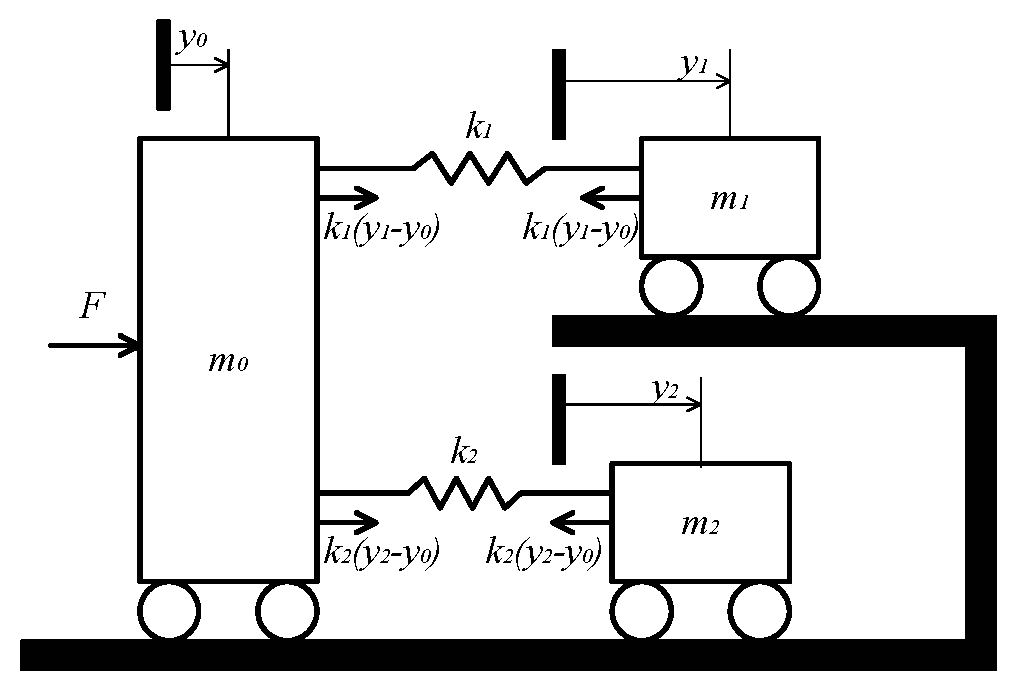
\includegraphics[width=0.7\linewidth]{sfigure/car3.eps}
 	\caption{３質量系}
	\label{fig_3mass}
 \end{center}
\end{figure}

\noindent

(hint) 3質量系の運動方程式は以下であらわされる．（$\ddot{y}=\frac{d^2y}{dt^2}$）
\begin{align}
	m_0 \ddot{y}_0 & = F + k_1 (y_1 - y_0) + k_2 (y_2-y_0)
\nonumber \\
	m_1 \ddot{y}_1 & = - k_1 (y_1 - y_0)
\nonumber \\
	m_2 \ddot{y}_2 & = - k_2 (y_2 - y_0)
\nonumber
\end{align}
\ \\

%%RC回路%%%%%%%%%%%%%%%%%%%%%%%%%%%%%%%%%%%%%%%%%%%%%%%%%%%%%%%%%%%%%%%
%	\noindent
%	{\bf ＜補助資料＞　電気回路　$RC$回路}

電気回路は$C$の電圧，$L$の電流を状態とすると状態方程式が求められる．
\begin{figure}[htbp]
 \begin{center}
%　
\epsfig{file=RC.eps,scale=1.5}
	\includegraphics[width=0.5\linewidth]{sfigure/RC.eps}
 	\caption{RC回路}
	\label{fig_RC}

 \end{center}
\end{figure}

例えばFig. \ref{fig_RC}の回路（入力:$v_i$, 出力:$v_o$）の方程式は
\begin{align*}
	v_R &= i R \\
	i & = C \frac{d v_C}{dt} \\
	v_i & = v_R + v_C \\
	v_o & = v_C
\end{align*}
となるが，状態を$v_C$（$C$の電圧）として，その微分を整理することにより以下の状態方程式が得られる．
\begin{align*}
	\frac{d v_C}{dt} 
	&= \frac{i}{C} 
	= \frac{v_R/R}{C} 
	= \frac{v_R}{RC} 
	= \frac{v_i - v_C}{RC} 
	= - \frac{1}{RC} v_C + \frac{1}{RC} v_i \\
	v_o & = v_C
\end{align*}
%---------------------------------------------------------------------------

%%LR回路%%%%%%%%%%%%%%%%%%%%%%%%%%%%%%%%%%%%%%%%%%%%%%%%%%%%%%%%%%%%%%%
%	\noindent
%	{\bf ＜補助資料＞　電気回路　$LR$回路}

\begin{figure}[htbp]
 \begin{center}
%　
\epsfig{file=LR.eps,scale=1.5}
	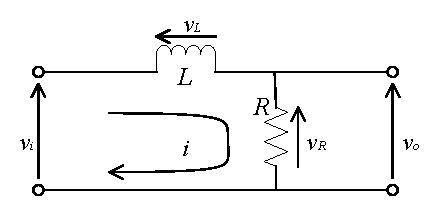
\includegraphics[width=0.5\linewidth]{sfigure/LR.eps}
 	\caption{LR回路}
	\label{fig_LR}
 \end{center}
\end{figure}

また，Fig. \ref{fig_LR}の回路の方程式は
\begin{align*}
	v_L & = L \frac{d i}{dt} \\
	v_R &= i R \\
	v_i & = v_L + v_R \\
	v_o & = v_R
\end{align*}
であり，状態を$i$（$L$の電流）として，その微分を整理することにより以下の状態方程式が得られる．
\begin{align*}
	\frac{d i}{dt} 
	&= \frac{v_L}{L} 
	= \frac{v_i - v_R}{L} 
	= - \frac{1}{L} v_R + \frac{1}{L} v_i 
	= - \frac{1}{L} R i + \frac{1}{L} v_i 
	= - \frac{R}{L} i + \frac{1}{L} v_i \\
	v_o & = v_R = R i
\end{align*}


%---------------------------------------------------------------------------

%%LCR回路%%%%%%%%%%%%%%%%%%%%%%%%%%%%%%%%%%%%%%%%%%%%%%%%%%%%%%%%%%%%%%%%%
\noindent
{\bf ＜演習＞ 電気回路　$LCR$回路}

以下の電気回路の状態方程式を求めよ（入力:$v_i$, 出力:$v_o$）．

\begin{figure}[htbp]
 \begin{center}
%　
\epsfig{file=LCR.eps,scale=1.5}
	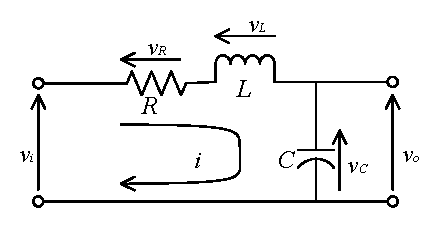
\includegraphics[width=0.5\linewidth]{sfigure/LCR.eps}
 	\caption{LCR回路}
	\label{fig_LCR}
 \end{center}
\end{figure}

\noindent
(hint)電気回路は$C$の電圧，$L$の電流を状態とすると状態方程式が求められる．
また，このLCR回路の方程式は以下で与えられる．
\begin{align*}
	v_L & = L \frac{d i}{dt} \\
	i & = C \frac{d v_C}{dt} \\
	v_R &= i R \\
	v_i & = v_L + v_C + v_R \\
	v_o & = v_C
\end{align*}



%---------------------------------------------------------------------------


\section{座標変換}\label{sec:zahyohenkan}
%---------------------------------------------------------------------------
システム(\ref{state_eq})(\ref{output_eq})における状態$x$はシステムの内部状
態を表わすもので，システムの入出力に直接には現われない．そこで，この状態
$x$を次のような{\bf {座標変換}(coordinate transformation)}で$\bar{x}$に変換することを考える．
\begin{equation}
 x = T \bar{x} \quad (\bar{x} = T^{-1}x)
\end{equation}
ここで$T$は正則な行列(nonsingular)であるとする．状態$\bar{x}$を時間微分(time derivative)すれば
\begin{align}
 \frac{d \bar{x}}{dt} &= T^{-1} \frac{dx}{dt} \nonumber \\
 &= T^{-1} ( A x + B u) \nonumber \\
 &= T^{-1} A T \bar{x} + T^{-1} B u \nonumber \\
 & \defeq \bar{A} \bar{x} + \bar{B} u
\label{eq:anotherstate_st}
\end{align}
なる状態方程式を得る．また出力方程式(output equation)は
\begin{align}
 y &= C T \bar{x} + D u \nonumber \\
   & \defeq \bar{C} \bar{x} + \bar{D} u
\label{eq:anotherstate_out}
\end{align}
となる．このように座標変換によりシステムの状態を変えても状態方程式でシス
テムの挙動を表わすことができる．
%---------------------------------------------------------------------------



\section{状態方程式から伝達関数へ}
%---------------------------------------------------------------------------
状態方程式(\ref{state_eq})において，
状態$x$, 入力$u$のラプラス変換を，
\begin{align}
 {\cal L}(x(t)) &=
 {\cal L} \left(
        \begin{array}{c}
	 x_1(t) \\
	 x_2(t)
	\end{array}
	\right) = 
 \left(
 \begin{array}{c}
  {\cal L}(x_1(t)) \\
  {\cal L}(x_2(t))
 \end{array}
 \right) = 
 \left(
 \begin{array}{c}
  X_1(s) \\
  X_2(s)
 \end{array}
 \right) = X(s) \\
 {\cal L}(u(t)) &= U(s)
\end{align}
とする．これを用いて
(\ref{state_eq})をラプラス変換し，$x$の初期値を$x(0) = 0$とおけば
\begin{eqnarray*}
 s X(s) = A X(s) + B U(s) & \Leftrightarrow & s X(s) - A X(s) = B U(s) \\
                          & \Leftrightarrow & (sI - A)X(s) = B U(s)
\end{eqnarray*}
\begin{equation}
 \therefore X(s) = (s I - A)^{-1} B U(s)
\end{equation}
を得る．同様に，
出力方程式(\ref{output_eq})を考えれば入力から出力までの伝達関数(transfer function)$G(s)$は
\begin{align}
 Y(s) &= C X(s) + D U(s) \nonumber \\
      &= C (s I - A)^{-1} B U(s) + D U(s) \nonumber \\
      &= \{ C ( s I - A )^{-1} B + D \} U(s) \\
      &\defeq G(s) U(s)
\end{align}
で表わされる．


例えば，状態方程式(\ref{eq:massstate})(\ref{eq:massoutput})で表された
バネ・質量・ダンパー系の伝達関数は
\begin{align}
 G(s)
 &= C (s I - A)^{-1} B \\
 &= \left(
     \begin{array}{cc}
      1 & 0 
     \end{array}
    \right)
    \left(
     \begin{array}{cc}
      s           & -1 \\
      \frac{k}{m} & s+\frac{c}{m}
     \end{array}
    \right)^{-1}
    \left(
     \begin{array}{c}
      0 \\
      \frac{1}{m}
     \end{array}
    \right) \nonumber \\
 &= \left(
     \begin{array}{cc}
      1 & 0 
     \end{array}
    \right)
    \left\{
     \frac{1}{s(s + \frac{c}{m})+\frac{k}{m}}
     \left(
     \begin{array}{cc}
      s+\frac{c}{m} & 1 \\
      -\frac{k}{m}  & s
     \end{array}
     \right)
    \right\}
    \left(
     \begin{array}{c}
      0 \\
      \frac{1}{m}
     \end{array}
    \right) \nonumber \\
 &= \frac{1}{s^2 + \frac{c}{m}s + \frac{k}{m}}
    \left(
     \begin{array}{cc}
      1 & 0 
     \end{array}
    \right)
    \left(
     \begin{array}{cc}
      s+\frac{c}{m} & 1 \\
      -\frac{k}{m}  & s
     \end{array}
    \right)
    \left(
     \begin{array}{c}
      0 \\
      \frac{1}{m}
     \end{array}
    \right) \nonumber \\
 &= \frac{1}{s^2 + \frac{c}{m}s + \frac{k}{m}}
    \left(
     \begin{array}{cc}
      1 & 0 
     \end{array}
    \right)
    \left(
     \begin{array}{c}
      \frac{1}{m} \\
      \frac{s}{m}
     \end{array}
    \right) \nonumber \\
 &= \frac{\frac{1}{m}}{s^2 + \frac{c}{m}s + \frac{k}{m}}
\end{align}
のように計算できる．

座標変換されたシステム(\ref{eq:anotherstate_st})(\ref{eq:anotherstate_out})の伝達関数が座標変換される前の伝達関数と等しくなることは次のように証明できる．
\begin{align}
 \bar{C} (sI - \bar{A})^{-1} \bar{B} + \bar{D} 
 &= CT (sI - T^{-1} A T )^{-1} T^{-1} B + D
\nonumber\\
 &= C T \{ T^{-1} (sI - A) T \}^{-1} T^{-1} B + D
\nonumber\\
 &= C T \{ T^{-1} (sI - A)^{-1} T \} T^{-1} B + D
\nonumber \\
 &= C (sI - A)^{-1} B + D
\end{align}
%---------------------------------------------------------------------------



\section{1入出力伝達関数から状態方程式へ \label{sec_canonical}}
%---------------------------------------------------------------------------

{\bf {一入出力}(SISO: single input single output)}の伝達関数
\begin{equation}
 G(s) =
  \frac{b_{n-1} s^{n-1} + b_{n-2} s^{n-2} + \cdots + b_1 s + b_0}
  {s^n + a_{n-1} s^{n-1} + a_{n-2} s^{n-2} + \cdots + a_1 s + a_0}
  + d
  \label{eq:G(s)}
\end{equation}
で表わされるシステムの状態空間表現は一意ではない（座標変換分の自由度がある）．ここでは状態フィードバックの設計に関連深い可制御正準形について紹介する．

伝達関数(\ref{eq:G(s)})は以下の状態方程式で表される．このシステムは{\bf {可制御正準形}(controller canonical form)}と呼ばれる（可制御性(controllability)という言葉の意味は後に定義する）
\begin{align}
 \frac{d}{dt}
  \left(\begin{array}{c}
         x_1 \\
	 x_2 \\
	 \vdots \\
	 x_{n-1} \\
	 x_n
	\end{array}\right)
  &=
  \left(\begin{array}{ccccc}
     0      & 1      & 0      & \cdots & 0 \\
	 0      & 0      & 1      & \ddots & \vdots \\
	 \vdots & \vdots & \ddots & \ddots & 0 \\
	 0      & 0      & \cdots & 0      & 1 \\
	 -a_0   & -a_1   & \cdots & -a_{n-2} & -a_{n-1}
	\end{array}\right)
  \left(\begin{array}{c}
	 x_1 \\
	 x_2 \\
	 \vdots \\
	 x_{n-1} \\
	 x_n
	\end{array}\right)
  +
  \left(\begin{array}{c}
         0 \\
	 0 \\
	 \vdots \\
	 0 \\
	 1
	\end{array}\right)
  u \label{eq:canoform}\\
y &=
 \left(\begin{array}{ccccc}
        b_0 & b_1 & \cdots & b_{n-2} & b_{n-1}
       \end{array}\right)
 \left(\begin{array}{c}
        x_1 \\
	x_2 \\
	\vdots \\
	x_{n-1} \\
	x_n
       \end{array}\right)
 + d u
\end{align}
これは以下のように証明できる．まず，$(sI-A)^{-1}$が
\begin{align}
 (sI-A)^{-1}
 &=
    \left(\begin{array}{ccccc}
     s      & -1     &  0     & \cdots &  0 \\
	 0      &  s     & -1     & \ddots &  \vdots \\
	 \vdots & \vdots & \ddots & \ddots &  0 \\
	 0      &  0     & \cdots & s      & -1 \\
	 a_0    &  a_1   & \cdots & a_{n-2}  &  s+a_{n-1}
	\end{array}\right)^{-1}
\nonumber\\
 &=
    \frac{1}{s^n + a_{n-1} s^{n-1}  + \cdots + a_0}
    \left(\begin{array}{ccccc}
        &    &        &    &  1 \\
	    &    &        &    &  s \\
	  * &  * & \cdots &  * &  \vdots \\
	    &    &        &    &  s^{n-2} \\
	    &    &        &    &  s^{n-1}
	\end{array}\right)
\end{align}
となることは$(sI-A)(sI-A)^{-1}=I$より
\begin{align}
    \left(\begin{array}{ccccc}
     s      & -1     &  0     & \cdots &  0 \\
	 0      &  s     & -1     & \ddots &  \vdots \\
	 \vdots & \vdots & \ddots & \ddots &  0 \\
	 0      &  0     & \cdots & s      & -1 \\
	 a_0    &  a_1   & \cdots & a_{n-2}  &  s+a_{n-1}
	\end{array}\right)
  &
    \left(\begin{array}{ccccc}
        &    &        &    &  1 \\
	    &    &        &    &  s \\
	  * &  * & \cdots &  * &  \vdots \\
	    &    &        &    &  s^{n-2} \\
	    &    &        &    &  s^{n-1}
	\end{array}\right)
    \frac{1}{s^n + a_{n-1} s^{n-1}  + \cdots + a_0}
\nonumber \\
 &=
    \left(\begin{array}{ccccc}
        &    &        &    &  0 \\
	    &    &        &    &  0 \\
	  * &  * & \cdots &  * &  \vdots \\
	    &    &        &    &  0 \\
	    &    &        &    &  1
	\end{array}\right)
\end{align}
となることから明らかである．よって，
\begin{align}
 C(sI-A)^{-1}B + D
 &=
 \frac{
    \left(\begin{array}{ccccc}
        b_0 & b_1 & \cdots & b_{n-2} & b_{n-1}
    \end{array}\right)
    \left(\begin{array}{ccccc}
        &    &        &    &  1 \\
	    &    &        &    &  s \\
	  * &  * & \cdots &  * &  \vdots \\
	    &    &        &    &  s^{n-2} \\
	    &    &        &    &  s^{n-1}
	\end{array}\right)
    \left(\begin{array}{c}
         0 \\
	 0 \\
	 \vdots \\
	 0 \\
	 1
	\end{array}\right)
 }
 {s^n + a_{n-1} s^{n-1}  + \cdots + a_0}
    + d
\nonumber\\[1cm]
 &=
 \frac{
    \left(\begin{array}{ccccc}
        b_0 & b_1 & \cdots & b_{n-2} & b_{n-1}
    \end{array}\right)
    \left(\begin{array}{c}
     1 \\
	 s \\
	 \vdots \\
	 s^{n-2} \\
	 s^{n-1}
	\end{array}\right)
 }
 {s^n + a_{n-1} s^{n-1}  + \cdots + a_0}
    + d
\nonumber \\[1cm]
 &=
   \frac{b_{n-1} s^{n-1} + b_{n-2} s^{n-2} + \cdots + b_1 s + b_0}
  {s^n + a_{n-1} s^{n-1} + a_{n-2} s^{n-2} + \cdots + a_1 s + a_0}
  + d
\end{align}
となる．

例えば，近似微分要素を表す伝達関数について確認してみると，
\begin{align}
 \frac{Ts}{Ts+1} = \frac{s}{s+\frac{1}{T}}
 = \frac{-\frac{1}{T}}{s+\frac{1}{T}} + 1
\end{align}
となるので，状態方程式で表すと
\begin{align}
 \frac{dx}{dt} &= -\frac{1}{T} x + 1u \\
 y             &= -\frac{1}{T} x + 1u
\end{align}
となる．

%---------------------------------------------------------------------------
\section{可制御性}
%---------------------------------------------------------------------------

\subsection{可制御性の定義}

状態方程式(\ref{state_eq})において初期状態$x(0)=x_0$を有限時間$t_1$で原点に移す$(x(t_1)=0)$入力$u(t), t\in[0,t_1]$が存在するとき$x_0$は{\bf 可制御(controllable)}であるという．また，すべての状態$x_0$が可制御であるとき，状態方程式は可制御であるという．可制御でない状態方程式は{\bf 不可制御(uncontrollable)}であるという．可制御性は$A,B$行列のみに依存する性質なので{\bf $(A,B)$可制御}ということもある．可制御性についての詳細な議論は成書に譲り，ここではシステムの分解の観点から直感的に理解することを考える．

\subsubsection{（行列論：復習）ランク}

ここで行列の階数を表す$\rank$は，与えられた行列における独立な列ベクトル(行ベクトル)の数である．例えば
\[
 \begin{array}{lcl}
  \rank
   \left(
    \begin{array}{cc}
     1 & 0 \\
     0 & 1 \\
     0 & 0
    \end{array}
   \right) = 2 & \Rightarrow & \mbox{1列目と2列目は独立なベクトル} \\
  \rank
   \left(
    \begin{array}{cc}
     1 & 2 \\
     0 & 0 \\
     0 & 0
    \end{array}
   \right) = 1 & \Rightarrow & \mbox{2列目は1列目を2倍したベクトル} \\
  \rank
   \left(
    \begin{array}{ccc}
     1 & 0 & 1 \\
     0 & 1 & 1\\
     0 & 0 & 0
    \end{array}
   \right) = 2 & \Rightarrow & \mbox{3列目は1列目と2列目の線形結合}
 \end{array}
\]

\subsubsection{（行列論：復習）ブロック行列}

ブロック行列：行列をブロックに分けて計算することがある．
\begin{equation*}
	A =
	\left(\begin{array}{ccc}
			a_{11} & a_{12} & a_{13}\\
			a_{21} & a_{22} & a_{23}\\
			a_{31} & a_{32} & a_{33}\\
			a_{41} & a_{42} & a_{43}
	\end{array}\right)
	=
	\left(\begin{array}{c|cc}
			a_{11} & a_{12} & a_{13}\\
			a_{21} & a_{22} & a_{23}\\
			\hline
			a_{31} & a_{32} & a_{33}\\
			a_{41} & a_{42} & a_{43}
	\end{array}\right)
	=
	\left(\begin{array}{cc}
		A_{11} & A_{12} \\
		A_{21} & A_{22}
	\end{array}\right)
\end{equation*}

ブロック行列の積：通常の行列と同様に計算できる．
\begin{equation*}
	\left(\begin{array}{cc}
		A_{11} & A_{12} \\
		A_{21} & A_{22}
	\end{array}\right)
	\left(\begin{array}{cc}
		B_{11} & B_{12} \\
		B_{21} & B_{22} \\
	\end{array}\right)
	=
	\left(\begin{array}{cc}
		A_{11} B_{11} + A_{12} B_{21} & A_{11} B_{12} + A_{12} B_{22} \\
		A_{21} B_{11} + A_{22} B_{21} & A_{21} B_{12} + A_{22} B_{22}
	\end{array}\right)
\end{equation*}
　　それぞれの行列の積と和が計算できるサイズのときのみ成立(例)
\begin{equation*}
	\left(\begin{array}{c|cc}
			a_{11} & a_{12} & a_{13}\\
			a_{21} & a_{22} & a_{23}\\
			\hline
			a_{31} & a_{32} & a_{33}\\
			a_{41} & a_{42} & a_{43}
	\end{array}\right)
	\left(\begin{array}{cc|c}
			b_{11} & b_{12} & b_{13}\\
			\hline
			b_{21} & b_{22} & b_{23}\\
			b_{31} & b_{32} & b_{33}
	\end{array}\right)
\end{equation*}

\subsection{不可制御な状態方程式}

次のシステムを考える．ここで
$x = \left(\begin{array}{c} {x}_1 \\ {x}_2 \end{array}\right) \in {\mathbb R}^n$, 
$x_1 \in {\mathbb R}^r$, $x_2 \in {\mathbb R}^{n-r}$で，$A,B,C$行列は$x$の分割にあわせて定義されているものとする（例えば$A_{11} \in {\mathbb R}^{r \times r}$, $A_{12} \in {\mathbb R}^{r \times (n-r)}$など）．

\begin{align}
 \frac{d}{dt}
  \left(\begin{array}{c}
         {x}_1 \\
	 {x}_2
	\end{array}\right)
  &=
  \left(\begin{array}{cc}
         {A}_{11} & {A}_{12} \\
	     {A}_{21} & {A}_{22}
	\end{array}\right)
  \left(\begin{array}{c}
         {x}_1 \\
	 {x}_2
	\end{array}\right)
  +
  \left(\begin{array}{c}
         {B}_1 \\
	 {B}_2
	\end{array}\right)
  u \\
 y &=
  \left(\begin{array}{cc}
         {C}_1 & {C}_2
	\end{array}\right)
  \left(\begin{array}{c}
         {x}_1 \\
	 {x}_2
	\end{array}\right)
  + D u
\end{align}
このシステムの状態の一部$x_2$が入力$u$の影響を受けない（制御できない）ための条件を考える．

このシステムを次のように書き下す．
\begin{align}
 \frac{dx_1}{dt} &= A_{11} x_1 + A_{12} x_2 + B_1 u
\label{eq:controllable01} \\
 \frac{dx_2}{dt} &= A_{21} x_1 + A_{22} x_2 + B_2 u
\label{eq:controllable02}
\end{align}
(\ref{eq:controllable02})において$dx_2/dt$が入力$u$の影響を受けないためには最低限$B_2=0$の必要がある．$B_2=0$とすると，状態方程式は以下のようになる．
\begin{align}
 \frac{d}{dt}
  \left(\begin{array}{c}
         {x}_1 \\
	 {x}_2 
	\end{array}\right)
  &=
  \left(\begin{array}{cc}
         {A}_{11} & {A}_{12} \\
	     {A}_{21} & {A}_{22}
	\end{array}\right)
  \left(\begin{array}{c}
         {x}_1 \\
	 {x}_2 
	\end{array}\right)
  +
  \left(\begin{array}{c}
         {B}_1 \\
	 0
	\end{array}\right)
  u \\
 y &=
  \left(\begin{array}{cc}
         {C}_1 & {C}_2 
	\end{array}\right)
  \left(\begin{array}{c}
         {x}_1 \\
	 {x}_2 
	\end{array}\right)
  + D u
\end{align}
このシステムを次のように書き下す．
\begin{align}
 \frac{dx_1}{dt} &= A_{11} x_1 + A_{12} x_2 + B_1 u
\label{eq:controllable1} \\
 \frac{dx_2}{dt} &= A_{21} x_1 + A_{22} x_2
\label{eq:controllable2}
\end{align}
(\ref{eq:controllable1})より，$x_1$は入力$u$の影響を受ける．(\ref{eq:controllable2})より$x_2$は直接は入力$u$の影響は受けないが，($u$の影響を受ける)$x_1$の影響を受けるので，間接的に入力$u$の影響を受けていることになる．

しかし，もし状態方程式の$A_{21}$部分が$0$行列であるとすれば
\begin{align}
 \frac{d}{dt}
  \left(\begin{array}{c}
         {x}_1 \\
	 {x}_2 
	\end{array}\right)
  &=
  \left(\begin{array}{cc}
         {A}_{11} & {A}_{12} \\
	     0        & {A}_{22}
	\end{array}\right)
  \left(\begin{array}{c}
         {x}_1 \\
	 {x}_2 
	\end{array}\right)
  +
  \left(\begin{array}{c}
         {B}_1 \\
	 0
	\end{array}\right)
  u 
\label{eq:uncontrollable1}\\
 y &=
  \left(\begin{array}{cc}
         {C}_1 & {C}_2 
	\end{array}\right)
  \left(\begin{array}{c}
         {x}_1 \\
	 {x}_2 
	\end{array}\right)
  + D u
\label{eq:uncontrollable2}
\end{align}
書き下すと
\begin{align}
  \left\{
    \begin{alignedat}{3}
    \frac{d x_1}{dt} &= A_{11} x_1 +&& A_{12}x_2 + B_{1} u\\
    \frac{d x_2}{dt} &= &&A_{22}x_2
    \end{alignedat}
  \right. \label{eq:uncontrollable3}
\end{align}
となり，$x_2$は入力$u$の影響を受けない（制御できない）ことがわかる（Fig.\ref{fig_controlability}）．さらに$x_2(0) \neq 0$の場合には有限時間$t_1$では$x_2(t_1)$は$0$にはならないことは明らかである．つまり，状態方程式は不可制御である．

明らかに(\ref{eq:uncontrollable1})(\ref{eq:uncontrollable2})で表されるシステムや，座標変換で(\ref{eq:uncontrollable1})(\ref{eq:uncontrollable2})に変換されるシステムは不可制御なシステムである．


\begin{figure}[t]
 \begin{center}
  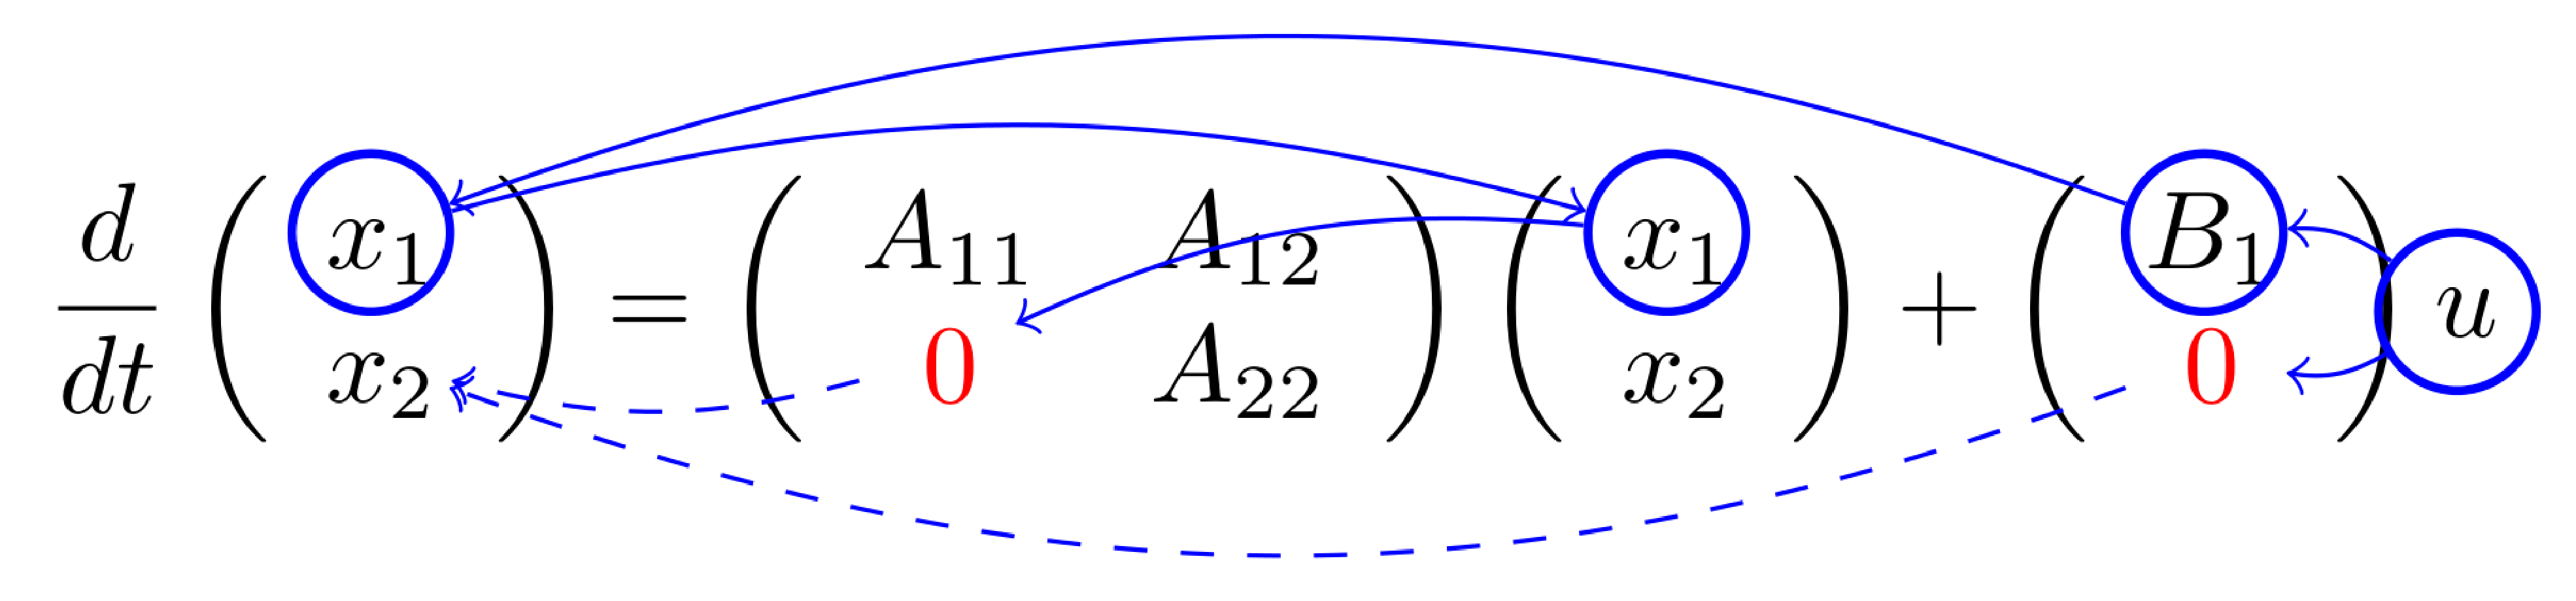
\includegraphics[width=0.7\linewidth]{sfigure/controlability.eps}
  \caption{不可制御なシステム}
  \label{fig_controlability}
 \end{center}
\end{figure}

\subsection{可制御性の条件}

不可制御なシステム(\ref{eq:uncontrollable1})(\ref{eq:uncontrollable2})について$V=(B,AB,\cdots, A^{n-1}B)$を計算してみよう．
\begin{align}
 V & = (B, AB, A^{2}B, \cdots, A^{n-1}B)
\nonumber \\
   & = \left[
          \begin{array}{ccccc}
             \left( 
                \begin{array}{c}
                   B_1 \\
                   0
                \end{array}
             \right)
             &
             \left( 
                \begin{array}{c}
                   A_{11} B_1 \\
                   0
                \end{array}
             \right)
             &
             \left( 
                \begin{array}{c}
                   A_{11}^2 B_1 \\
                   0
                \end{array}
             \right)
             &
             \cdots
             &
             \left( 
                \begin{array}{c}
                   A_{11}^{n-1} B_1 \\
                   0
                \end{array}
             \right)
          \end{array} 
       \right]
\end{align}
$x \in {\mathbb R}^n$, $ u \in {\mathbb R}^m $より$A\in {\mathbb R}^{n \times n}$, $B \in {\mathbb R}^{n \times m}$であるから$V \in {\mathbb R}^{n \times nm}$であるが，$x_2$にあたる下の$n-r$列が$0$である．これは
\begin{align}
 \mbox{rank}\ V &= \mbox{rank}  (B, AB, A^{2}B, \cdots, A^{n-1}B) \leq r < n
\end{align}
であることを示している．

不可制御なシステム(\ref{eq:uncontrollable1})(\ref{eq:uncontrollable2})を$\bar{A}= T^{-1} A T$, $\bar{B} = T^{-1}B$と座標変換したシステムについても$\bar{V}=(\bar{B},\bar{A}\bar{B},\cdots, \bar{A}^{n-1}\bar{B})$を計算してみると
\begin{align}
 \bar{V}&=(\bar{B},\bar{A}\bar{B},\bar{A}^{2}\bar{B},\cdots, \bar{A}^{n-1}\bar{B})
\nonumber\\
 &= [(T^{-1}B), (T^{-1}AT)(T^{-1}B),(T^{-1}AT)^{2}(T^{-1}B),\cdots,(T^{-1}AT)^{n-1}(T^{-1}B)]
\nonumber \\
 &= [T^{-1}B, T^{-1} AB, T^{-1} A^2 B,\cdots, T^{-1} A^{n-1} B]
\nonumber\\
 &= T^{-1} [B, AB, A^2 B,\cdots, A^{n-1} B]
\nonumber \\
 &= T^{-1} V
\end{align}
となり，$T^{-1}$が正則であることから
\begin{align}
 \mbox{rank}\ \bar{V} & = \mbox{rank}\ {V} \leq r < n
\end{align}
となる．これは
\begin{quote}
{\bf 不可制御なシステム(\ref{eq:uncontrollable1})(\ref{eq:uncontrollable2})に座標変換で変換できるシステムは\\
$\mbox{rank}\ V = \mbox{rank} (B,AB,\cdots,A^{n-1}B) < n$}
\end{quote}
となることを示している．逆に，
\begin{quote}
{\bf $\mbox{rank}\ V = \mbox{rank} (B,AB,\cdots,A^{n-1}B) < n$を満たすシステムは\\
不可制御なシステム(\ref{eq:uncontrollable1})(\ref{eq:uncontrollable2})に座標変換で変換できる．}
\end{quote}
ことが分かっている（次節）．つまり，
\begin{quote}
{\bf システムが不可制御なシステム(\ref{eq:uncontrollable1})(\ref{eq:uncontrollable2})に座標変換で変換できるための必要十条件は
$\mbox{rank}\ V = \mbox{rank} (B,AB,\cdots,A^{n-1}B) < n$}
\end{quote}
となる．これは不可制御なシステムに関する考察であるが，可制御性に関しては
\begin{quote}
{\bf システムが可制御であるための必要十分条件は\\
$\mbox{rank}\ V = \mbox{rank} (B,AB,\cdots,A^{n-1}B) = n$}
\end{quote}
が成り立つことがわかっている．このように$V$は可制御性を判断するために重要な役割を果たすので，$V$は{\bf 可制御性行列(controllability matrix)}と呼ばれている．
\\




\subsection{不可制御なシステムの分解 \label{sec:controllability_decomp}}

システムが可制御でないとき，つまり
\begin{equation}
 \rank V = r < n
\end{equation}
のときを考える．このとき$V$の列ベクトルの中から線形独立なもの$r$本を選び
これを$v_1, v_2, \cdots, v_r$と定義する．また$n-r$本の列ベクトル
$v_{r+1}, v_{r+2}, \cdots, v_n$を
\begin{equation}
 T = \left(\begin{array}{ccccccc}
            v_1 & v_2 & \cdots & v_r & v_{r+1} & \cdots & v_n
	   \end{array}\right)
\end{equation}
が正則になるように選び，簡単な代数計算を行うことでこの行列$T$により
座標変換されたシステムが
\begin{align}
 \frac{d}{dt}
  \left(\begin{array}{c}
         \bar{x}_1 \\
	 \bar{x}_2 
	\end{array}\right)
  &=
  \left(\begin{array}{cc}
         \bar{A}_{11} & \bar{A}_{12} \\
	 0            & \bar{A}_{22}
	\end{array}\right)
  \left(\begin{array}{c}
         \bar{x}_1 \\
	 \bar{x}_2 
	\end{array}\right)
  +
  \left(\begin{array}{c}
         \bar{B}_1 \\
	 0
	\end{array}\right)
  u \\
 y &=
  \left(\begin{array}{cc}
         \bar{C}_1 & \bar{C}_2 
	\end{array}\right)
  \left(\begin{array}{c}
         \bar{x}_1 \\
	 \bar{x}_2 
	\end{array}\right)
  + D u
\end{align}
% ここで，
% \begin{align}
%   \begin{array}{cc}
%     \left(
%       \begin{array}{c}
%         \bar x_1 \\ \bar x_2
%       \end{array}
%     \right)\in \mathbb{R}^{n} &
%     \begin{aligned}
%       \bar x_1 \in& \mathbb{R}^r \\
%       \bar x_2 \in& \mathbb{R}^{n-r} \\
%     \end{aligned}
%   \end{array}
% \end{align}
と表わされることが示される．


例えば，以下のようなシステム
\begin{equation}
 \frac{d}{dt}
  \left(
   \begin{array}{c}
    x_1 \\
    x_2
   \end{array}
  \right) = 
  \left(
   \begin{array}{cc}
    1 & 0 \\
    0 & 1
   \end{array}
  \right)
  \left(
   \begin{array}{c}
    x_1 \\
    x_2
   \end{array}
  \right) +
  \left(
   \begin{array}{c}
    1 \\
    1
   \end{array}
  \right) u
\end{equation}
において，可制御性行列$V$は
\begin{equation}
 V = 
  \left(
   \begin{array}{cc}
    B & AB\\
   \end{array}
  \right) =
  \left(
   \begin{array}{cc}
    1 & 1 \\
    1 & 1
   \end{array}
  \right)
\end{equation}
となり，明らかに$\rank V = 1$であるので，このシステムは可制御ではない．
ここで，$v_1 = (\begin{array}{cc}1 & 1\end{array})^T$, 
$v_2 = (\begin{array}{cc}0 & 1\end{array})^T$と選ぶことで，
\begin{equation}
 \begin{array}{cc}
  T =
   \left(
    \begin{array}{cc}
     1 & 0 \\
     1 & 1
    \end{array}
   \right),
   & 
  T^{-1} =
   \left(
    \begin{array}{cc}
     1 & 0 \\
     -1 & 1
    \end{array}
   \right)
 \end{array}
\end{equation}
のように正則な行列$T$を選ぶことができる．
この$T$により座標変換を行うと，
\begin{align}
 \bar{A} &= T^{-1}AT =
 \left(
 \begin{array}{cc}
  1 & 0 \\
  -1 & 0
 \end{array}
 \right)
 \left(
 \begin{array}{cc}
  1 & 0 \\
  0 & 1
 \end{array}
 \right)
 \left(
 \begin{array}{cc}
  1 & 0 \\
  1 & 1
 \end{array}
 \right) =
 \left(
 \begin{array}{cc}
  1 & 0 \\
  0 & 1
 \end{array}
 \right) \\
 \bar{B} &= T^{-1}B =
 \left(
 \begin{array}{cc}
  1 & 0 \\
  -1 & 1
 \end{array}
 \right)
 \left(
 \begin{array}{c}
  1 \\
  1 
 \end{array}
 \right) =
 \left(
 \begin{array}{c}
  1 \\
  0 
 \end{array}
 \right)
\end{align}
となるので，座標変換後のシステム
\begin{equation}
 \frac{d}{dt}
  \left(
   \begin{array}{c}
    \bar{x}_1 \\
    \bar{x}_2
   \end{array}
  \right) = 
  \left(
   \begin{array}{cc}
    1 & 0 \\
    0 & 1
   \end{array}
  \right)
  \left(
   \begin{array}{c}
    \bar{x}_1 \\
    \bar{x}_2
   \end{array}
  \right) +
  \left(
   \begin{array}{c}
    1 \\
    0
   \end{array}
  \right) u
\end{equation}
では確かに状態$\bar{x}_2$は入力$u$の影響を受けていない．
\\

\noindent
{\bf ＜演習＞ ３質量系の可制御性}\nopagebreak

Fig.\ref{fig_3mass}で用いた３質量系の状態方程式は
\begin{align}
 \frac{d}{dt} \left(\begin{array}{c}
	         y_0 \\
		     y_1 \\
		     y_2 \\
		     \frac{dy_0}{dt} \\
		     \frac{dy_1}{dt} \\
		     \frac{dy_2}{dt}
		    \end{array}\right)
 &=
 \left(\begin{array}{cccccc}
        0 & 0 & 0 & 1 & 0 & 0      \\
        0 & 0 & 0 & 0 & 1 & 0      \\
        0 & 0 & 0 & 0 & 0 & 1      \\
	-\frac{k_1}{m_0} -\frac{k_2}{m_0}&  \frac{k_1}{m_0} &  \frac{k_2}{m_0} & 0 & 0 & 0 \\
	 \frac{k_1}{m_1}                & -\frac{k_1}{m_1} &  0               & 0 & 0 & 0 \\
	 \frac{k_2}{m_2}                &  0               & -\frac{k_2}{m_2} & 0 & 0 & 0 
       \end{array}\right)
 \left(\begin{array}{c}
	         y_0 \\
		     y_1 \\
		     y_2 \\
		     \frac{dy_0}{dt} \\
		     \frac{dy_1}{dt} \\
		     \frac{dy_2}{dt}
       \end{array}\right)
 +
 \left(\begin{array}{c}
        0 \\
        0 \\
        0 \\
	    \frac{1}{m_0} \\
	    0 \\
	    0 
       \end{array}\right)
        F
\nonumber
\\
 \left(\begin{array}{c}
	    y_0 \\
		y_1 \\
		y_2
       \end{array}\right)
 &=
 \left(\begin{array}{cccccc}
         1 & 0 & 0 & 0 & 0 & 0  \\
         0 & 1 & 0 & 0 & 0 & 0 \\
         0 & 0 & 1 & 0 & 0 & 0 \\
       \end{array}\right)
 \left(\begin{array}{c}
	         y_0 \\
		     y_1 \\
		     y_2 \\
		     \frac{dy_0}{dt} \\
		     \frac{dy_1}{dt} \\
		     \frac{dy_2}{dt}
       \end{array}\right)
\nonumber
\end{align}
となる．このシステムについて以下を確認せよ．

・$m_0=m_1=m_2=1$, $k_1=k_2=1$のとき，システムは不可制御

・$m_0=m_1=m_2=1$, $k_1=1$, $k_2=2$のとき，システムは可制御
\\

\noindent
{\bf ＜演習＞不可制御なシステムの分解} \nopagebreak

次のシステムが不可制御であることを確認し，可制御な部分と不可制御な部分に分けよ．\begin{align*}
	\frac{d}{dt}
	\left (
	\begin{array}{c}
	 x_1 \\ x_2 
	\end{array}
	\right )
	& = 
	\left (
	\begin{array}{cc}
	 0 & 1 \\
	 -1 & 2
	\end{array}
	\right )
	\left (
	\begin{array}{c}
	 x_1 \\ x_2 
	\end{array}
	\right )
	+
	\left (
	\begin{array}{c}
	 1 \\ 1 
	\end{array}
	\right )
	u
\\
	y 
	&=
	\left (
	\begin{array}{cc}
	 1 & 1  
	\end{array}
	\right )
	\left (
	\begin{array}{c}
	 x_1 \\ x_2 
	\end{array}
	\right )
\end{align*}




%---------------------------------------------------------------------------
\section{可観測性}
%---------------------------------------------------------------------------

\subsection{可観測性の定義}

システム(\ref{state_eq})(\ref{output_eq})において，有限時間$[0,t_1]$の入力$u(t),0 \leq t \leq t_1$と出力$y(t), 0 \leq t \leq t_1$から初期状態$x(0)=x_0$を一意に決定できるとき，システムは{\bf 可観測(observable)}であるという．後に述べるように，システムの{\bf 可観測性(observability)}は$C,A$行列のみで決定されるので，{\bf $(C,A)$可観測}と呼ばれることもある．

可観測とはシステムの入出力から状態が推定できるか否かという概念である．厳密な解析は成書に譲り，ここではシステムの分解を用いて直感的に理解しよう．

\subsection{不可観測な状態方程式}

次のシステムを考える．ここで
$x = \left(\begin{array}{c} {x}_1 \\ {x}_2 \end{array}\right) \in {\mathbb R}^n$, 
$x_1 \in {\mathbb R}^r$, $x_2 \in {\mathbb R}^{n-r}$で，$A,B,C$行列は$x$の分割にあわせて定義されているものとする（例えば$A_{11} \in {\mathbb R}^{r \times r}$, $A_{12} \in {\mathbb R}^{r \times (n-r)}$など）．
\begin{align}
 \frac{d}{dt}
  \left(\begin{array}{c}
         {x}_1 \\
   {x}_2
  \end{array}\right)
  &=
  \left(\begin{array}{cc}
         {A}_{11} & {A}_{12} \\
       {A}_{21} & {A}_{22}
  \end{array}\right)
  \left(\begin{array}{c}
         {x}_1 \\
   {x}_2
  \end{array}\right)
  +
  \left(\begin{array}{c}
         {B}_1 \\
   {B}_2
  \end{array}\right)
  u \\
 y &=
  \left(\begin{array}{cc}
         {C}_1 & C_2
  \end{array}\right)
  \left(\begin{array}{c}
         {x}_1 \\
   {x}_2
  \end{array}\right)
  + D u
\end{align}
このシステムを次のように書き下す．
\begin{align}
 \frac{dx_1}{dt} &= A_{11} x_1 + A_{12} x_2 + B_1 u
\label{eq:observable1} \\
 \frac{dx_2}{dt} &= A_{21} x_1 + A_{22} x_2 + B_2 u
\label{eq:observable2} \\
 y & = C_1 x_1 + C_2 x_2+ Du
\label{eq:observable03}
\end{align}
このシステムの状態$x_2$が出力$y$から見えない（観測できない）ためには$C_2=0$である必要がある．$C_2=0$とすると状態方程式は以下となる．
\begin{align}
 \frac{d}{dt}
  \left(\begin{array}{c}
         {x}_1 \\
	 {x}_2 
	\end{array}\right)
  &=
  \left(\begin{array}{cc}
         {A}_{11} & {A}_{12} \\
	     {A}_{21} & {A}_{22}
	\end{array}\right)
  \left(\begin{array}{c}
         {x}_1 \\
	 {x}_2 
	\end{array}\right)
  +
  \left(\begin{array}{c}
         {B}_1 \\
	 {B}_2
	\end{array}\right)
  u \\
 y &=
  \left(\begin{array}{cc}
         {C}_1 & 0
	\end{array}\right)
  \left(\begin{array}{c}
         {x}_1 \\
	 {x}_2 
	\end{array}\right)
  + D u
\end{align}
このシステムを次のように書き下す．
\begin{align}
 \frac{dx_1}{dt} &= A_{11} x_1 + A_{12} x_2 + B_1 u
\label{eq:observable1} \\
 \frac{dx_2}{dt} &= A_{21} x_1 + A_{22} x_2 + B_2 u
\label{eq:observable2} \\
 y & = C_1 x_1 + Du
\label{eq:observable3}
\end{align}
(\ref{eq:observable3})より，出力$y$は$x_1$の影響を受ける．出力$y$は$x_2$の影響を直接は受けないが，(\ref{eq:observable1})より$x_1$が$x_2$の影響を受けるため，間接的に$x_2$も$y$に影響する可能性がある．つまり，このシステムでは$x_1$も$x_2$も出力に影響を与える可能性がある．言い換えれば出力$y$は$x_1,x_2$の両方の情報を持っているので，なんらか手法で出力$y$から状態$x = \left(\begin{array}{c} {x}_1 \\ {x}_2 \end{array}\right)$を決定できる可能性を持っている．しかし，もし，この状態方程式の$A_{12}$の部分が$0$行列であるとすれば
\begin{align}
 \frac{d}{dt}
  \left(\begin{array}{c}
         {x}_1 \\
	 {x}_2 
	\end{array}\right)
  &=
  \left(\begin{array}{cc}
         {A}_{11} & 0 \\
	     {A}_{21} & {A}_{22}
	\end{array}\right)
  \left(\begin{array}{c}
         {x}_1 \\
	 {x}_2 
	\end{array}\right)
  +
  \left(\begin{array}{c}
         {B}_1 \\
	 {B}_2
	\end{array}\right)
  u 
\label{eq:unobservable1} \\
 y &=
  \left(\begin{array}{cc}
         {C}_1 & 0
	\end{array}\right)
  \left(\begin{array}{c}
         {x}_1 \\
	 {x}_2 
	\end{array}\right)
  + D u
\label{eq:unobservable2}
\end{align}
であり，書き下すと
\begin{align}
 \frac{dx_1}{dt} &= A_{11} x_1 \ \ \ \ \ \ \ \ \ \ \ + B_1 u
\label{eq:unobservable3} \\
 \frac{dx_2}{dt} &= A_{21} x_1 + A_{22} x_2 + B_2 u
\label{eq:unobservable4} \\
 y & = C_1 x_1 + Du
\label{eq:unobservable5}
\end{align}
となる．この場合，(\ref{eq:unobservable5})より出力$y$は$x_1$の影響を受けるが，$x_2$の影響は直接は受けない．また(\ref{eq:unobservable3})より$x_1$も$x_2$の影響を受けないため，最終的に出力$y$は$x_2$の影響をまったく受けなくなってしまう（Fig.\ref{fig_observability}）．つまり，出力$y$は$x_2$の情報を持たないため，何をしても出力（と入力）から$x_2$を決定することができない．つまり不可観測なシステムであることがわかる．

明らかに(\ref{eq:unobservable1})(\ref{eq:unobservable2})で表されるシステムや，座標変換で(\ref{eq:unobservable1})(\ref{eq:unobservable2})に変換されるシステムは不可観測なシステムである．

\begin{figure}[t]
 \begin{center}
  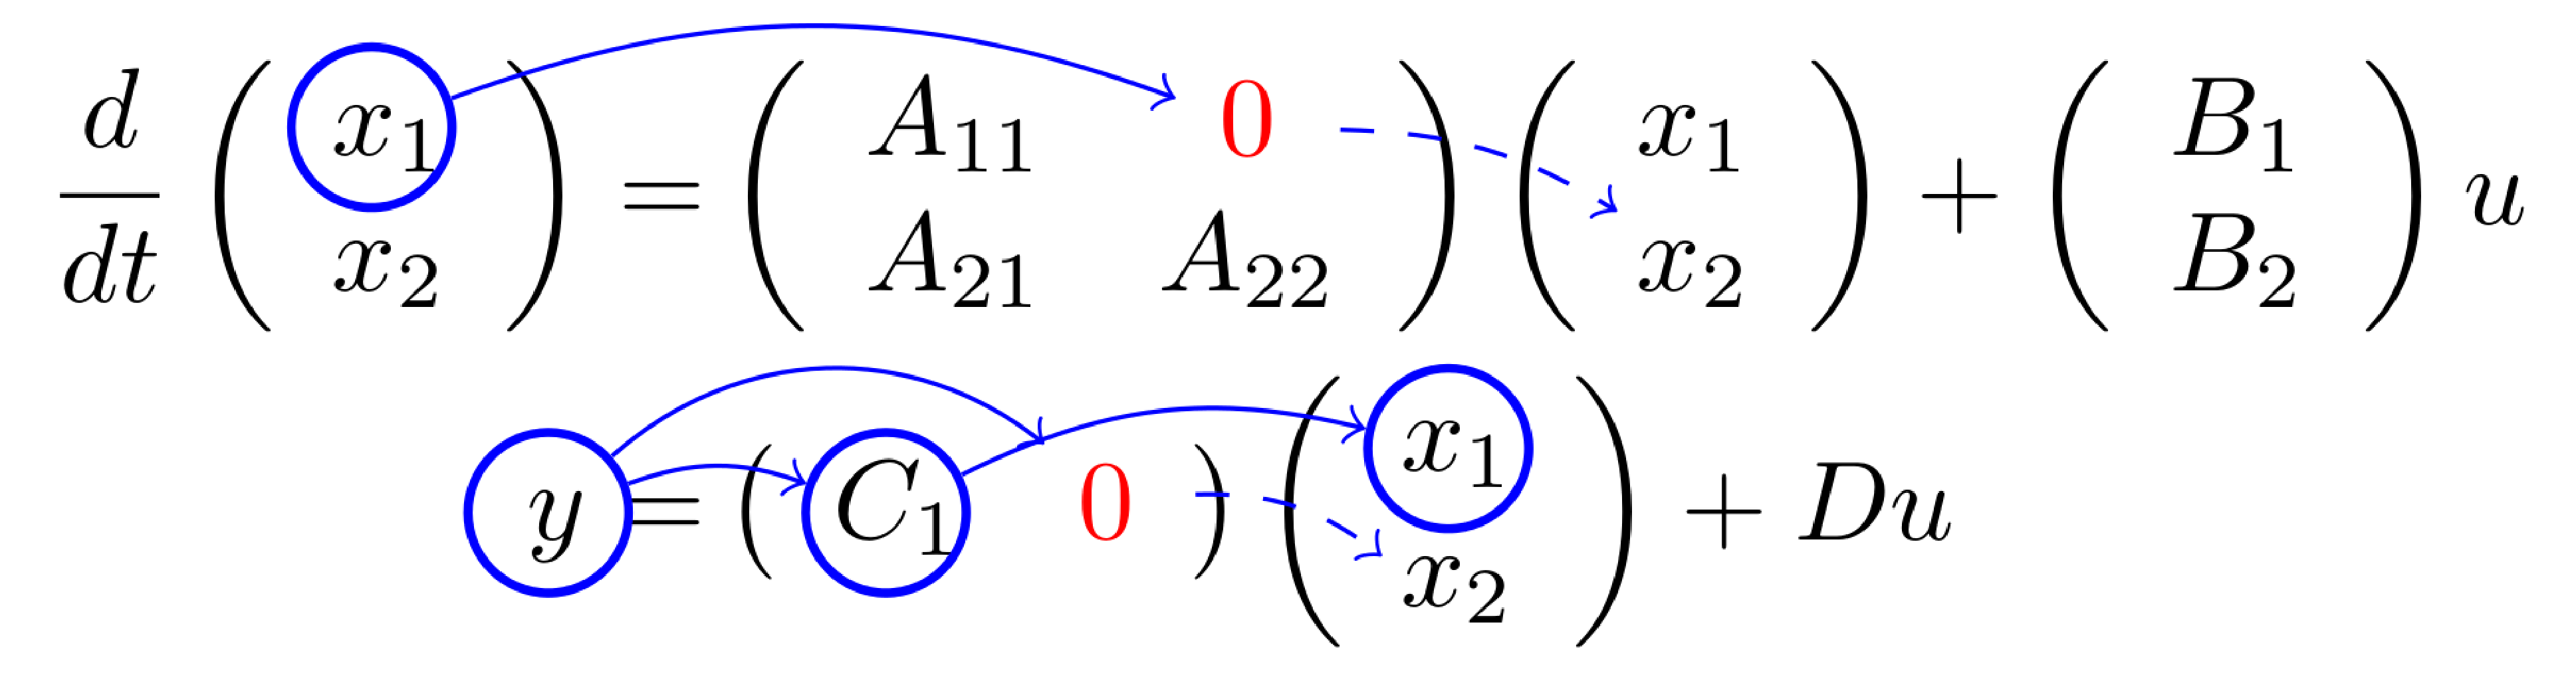
\includegraphics[width=0.7\linewidth]{sfigure/observability.eps}
  \caption{不可観測なシステム}
  \label{fig_observability}
 \end{center}
\end{figure}


\subsection{可観測性の条件}

不可観測なシステム(\ref{eq:unobservable1})(\ref{eq:unobservable2})について
\begin{equation}
 N^T =
  \left(\begin{array}{c}
         C        \\
	 C A      \\
	 C A^2    \\
	 \vdots   \\
	 C A^{n-1}
	\end{array}\right)
\end{equation}
を計算してみると
\begin{equation}
 N^T =
  \left(\begin{array}{c}
         C        \\
	 C A      \\
	 C A^2    \\
	 \vdots   \\
	 C A^{n-1}
	\end{array}\right)
 =
  \left(\begin{array}{lr}
	     (C_1           & 0) \\
		 (C_1 A_{11}       & 0) \\
		 (C_1 A_{11}^2     & 0) \\
		 \vdots   \\
		 (C_1 A_{11}^{n-1} & 0)
  \end{array}\right)
\end{equation}
となる．$x \in {\mathbb R}^n$, $ y \in {\mathbb R}^p $より$A\in {\mathbb R}^{n \times n}$, $C \in {\mathbb R}^{p \times n}$であるから$N^T \in {\mathbb R}^{np \times n}$であるが，$x_2$にあたる右側の$n-r$列が$0$である．これは
\begin{align}
 \mbox{rank}\ N^T 
 &= \mbox{rank} 
  \left(\begin{array}{c}
         C        \\
	 C A      \\
	 C A^2    \\
	 \vdots   \\
	 C A^{n-1}
	\end{array}\right)
   \leq r < n
\end{align}
であることを示している．

不可観測なシステム(\ref{eq:unobservable1})(\ref{eq:unobservable2})を$\bar{A}= T^{-1} A T$, $\bar{C} = C T$と座標変換したシステムについても同様に$\bar{N}^T$を計算してみると
\begin{align}
 \bar{N}^T 
 &= 
  \left(\begin{array}{c}
     \bar{C}        \\
	 \bar{C} \bar{A}      \\
	 \bar{C} \bar{A}^2    \\
	 \vdots   \\
	 \bar{C} \bar{A}^{n-1}
	\end{array}\right)
 = 
  \left(\begin{array}{c}
     CT        \\
	 CT T^{-1}AT      \\
	 CT T^{-1}A^2T    \\
	 \vdots   \\
	 CT T^{-1}A^{n-1}T
	\end{array}\right)
 =
  \left(\begin{array}{c}
     C T       \\
	 C A T     \\
	 C A^2 T   \\
	 \vdots   \\
	 C A^{n-1}T
	\end{array}\right)
 =
  \left(\begin{array}{c}
         C        \\
	 C A      \\
	 C A^2    \\
	 \vdots   \\
	 C A^{n-1}
	\end{array}\right)
	T
\nonumber \\
 &= N^T T
\end{align}
となり，$T$が正則であることから
\begin{align}
 \mbox{rank}\ \bar{N^T} & = \mbox{rank}\ {N^T} \leq r < n
\end{align}
となる．これは
\begin{quote}
   {\bf 不可観測なシステム(\ref{eq:unobservable1})(\ref{eq:unobservable2})に座標変換で
   変換できるシステムは\\
   $\mbox{rank}\ N^T 
   = \mbox{rank} 
	  \left(\begin{array}{c}
	         C        \\
		 C A      \\
		 C A^2    \\
		 \vdots   \\
		 C A^{n-1}
		\end{array}\right)
    < n$}
\end{quote}
となることを示している．逆に
\begin{quote}
   {\bf    $\mbox{rank}\ N^T 
   = \mbox{rank} 
	  \left(\begin{array}{c}
	         C        \\
		 C A      \\
		 C A^2    \\
		 \vdots   \\
		 C A^{n-1}
		\end{array}\right)
    < n$を満たすシステムは不可観測なシステム(\ref{eq:unobservable1})(\ref{eq:unobservable2})に座標変換で変換できる．}
\end{quote}
ことが分かっている（次節）．つまり，
\begin{quote}
   {\bf システムが不可観測なシステム(\ref{eq:unobservable1})(\ref{eq:unobservable2})に座標変換で変換できるための必要十分条件は
   $\mbox{rank}\ N^T 
   = \mbox{rank} 
	  \left(\begin{array}{c}
	         C        \\
		 C A      \\
		 C A^2    \\
		 \vdots   \\
		 C A^{n-1}
		\end{array}\right)
    < n$}
\end{quote}
となる．これは不可観測なシステムに対する考察であるが，可観測に関しては
\begin{quote}
	{\bf システムが可観測であるための必要十分条件は
	$\mbox{rank}\ N^T 
	= \mbox{rank} 
	  \left(\begin{array}{c}
	         C        \\
		 C A      \\
		 C A^2    \\
		 \vdots   \\
		 C A^{n-1}
		\end{array}\right)
	= n$}
\end{quote}
が成り立つことがわかっている．このように$N$は可観測性を判断するために重要な役割を果たすので，$N$は{\bf 可観測性行列(observability matrix)}と呼ばれている



\subsection{不可観測性なシステムの分解 \label{sec:observability_decomp}}

システムが可観測でないとき，つまり
\begin{equation}
 \rank N^T = r < n
\end{equation}
のときを考える．このとき$N^T$の行ベクトルの中から線形独立なもの$r$本を選
びこれを$w_1^T, w_2^T, \cdots, w_r^T$と定義する．また$n-r$本の行ベ
クトル$w_{r+1}^T, w_{r+2}^T, \cdots, w_n^T$を
\begin{equation}
 W = \left(\begin{array}{c}
            w_1^T \\
	    w_2^T \\
	    \vdots \\
	    w_r^T \\
	    w_{r+1}^T \\
	    \vdots \\
	    w_n^T
	   \end{array}\right)
\end{equation}
が正則になるように選ぶ．さらに$T=W^{-1}$とすると簡単な代数計算によりこの
行列$T$により座標変換されたシステムが
\begin{align}
 \frac{d}{dt}
  \left(\begin{array}{c}
         \bar{x}_1 \\
	 \bar{x}_2 
	\end{array}\right)
  &=
  \left(\begin{array}{cc}
         \bar{A}_{11} & 0 \\
	 \bar{A}_{21} & \bar{A}_{22}
	\end{array}\right)
  \left(\begin{array}{c}
         \bar{x}_1 \\
	 \bar{x}_2 
	\end{array}\right)
  +
  \left(\begin{array}{c}
         \bar{B}_1 \\
	 \bar{B}_2
	\end{array}\right)
  u \\
 y &=
  \left(\begin{array}{cc}
         \bar{C}_1 & 0         
	\end{array}\right)
  \left(\begin{array}{c}
         \bar{x}_1 \\
	 \bar{x}_2 
	\end{array}\right)
  + D u
\end{align}
と表わされることが分かる．

例えば，先と同じ以下のようなシステムを考える．
\begin{align}
 \frac{d}{dt}
  \left(
   \begin{array}{c}
    x_1 \\
    x_2
   \end{array}
  \right) &= 
  \left(
   \begin{array}{cc}
    1 & 0 \\
    0 & 1
   \end{array}
  \right)
  \left(
   \begin{array}{c}
    x_1 \\
    x_2
   \end{array}
  \right) +
  \left(
   \begin{array}{c}
    1 \\
    1
   \end{array}
  \right) u \\
 y &=
  \left(
   \begin{array}{cc}
    1 & 1
   \end{array}
  \right) 
  \left(
   \begin{array}{c}
    x_1 \\
    x_2
   \end{array}
  \right)
\end{align}
このとき，可観測性行列$N$は
\begin{equation}
 N^T = 
  \left(
   \begin{array}{c}
    C \\
    CA
   \end{array}
  \right) =
  \left(
   \begin{array}{cc}
    1 & 1 \\
    1 & 1
   \end{array}
  \right)
\end{equation}
となり，明らかに$\rank N = 1$であるので，このシステムは可観測ではない．
ここで，$w_1^T = (\begin{array}{cc}1 & 1\end{array})$, 
$w_2^T = (\begin{array}{cc}0 & 1\end{array})$と選ぶことで，
\begin{equation}
 \begin{array}{cc}
  W =
   \left(
    \begin{array}{cc}
     1 & 1 \\
     0 & 1
    \end{array}
   \right),
   & 
  W^{-1} =
   \left(
    \begin{array}{cc}
     1 & -1 \\
     0 & 1
    \end{array}
   \right)
 \end{array}
\end{equation}
のように正則な行列$W$を選ぶことができる．
この$W^{-1} = T$により座標変換を行うと，
\begin{align}
 \bar{A} &= T^{-1}AT =
 \left(
 \begin{array}{cc}
  1 & 1 \\
  0 & 1
 \end{array}
 \right)
 \left(
 \begin{array}{cc}
  1 & 0 \\
  0 & 1
 \end{array}
 \right)
 \left(
 \begin{array}{cc}
  1 & -1 \\
  0 & 1
 \end{array}
 \right) =
 \left(
 \begin{array}{cc}
  1 & 0 \\
  0 & 1
 \end{array}
 \right) \\
 \bar{B} &= T^{-1}B =
 \left(
 \begin{array}{cc}
  1 & 1 \\
  0 & 1
 \end{array}
 \right)
 \left(
 \begin{array}{c}
  1 \\
  1 
 \end{array}
 \right) =
 \left(
 \begin{array}{c}
  2 \\
  1 
 \end{array}
 \right) \\
 \bar{C} &= CT =
 \left(
 \begin{array}{cc}
  1 & 1
 \end{array}
 \right) 
 \left(
 \begin{array}{cc}
  1 & -1 \\
  0 & 1
 \end{array}
 \right) = 
 \left(
 \begin{array}{cc}
  1 & 0
 \end{array}
 \right) 
\end{align}
となるので，座標変換後のシステム
\begin{align}
 \frac{d}{dt}
  \left(
   \begin{array}{c}
    \bar{x}_1 \\
    \bar{x}_2
   \end{array}
  \right) &= 
  \left(
   \begin{array}{cc}
    1 & 0 \\
    0 & 1
   \end{array}
  \right)
  \left(
   \begin{array}{c}
    \bar{x}_1 \\
    \bar{x}_2
   \end{array}
  \right) +
  \left(
   \begin{array}{c}
    2 \\
    1
   \end{array}
  \right) u \\
 y &=
  \left(
   \begin{array}{cc}
    1 & 0
   \end{array}
  \right) 
  \left(
   \begin{array}{c}
    \bar{x}_1 \\
    \bar{x}_2
   \end{array}
  \right)
\end{align}
では確かに出力$y$は状態$\bar{x}_2$の影響を受けていない．
\\

\noindent
{\bf ＜演習＞３質量系の可観測性}

Fig.\ref{fig_3mass}の３質量系で，出力が$y=y_0$の場合，状態方程式と出力方程式は
\begin{align}
 \frac{d}{dt} \left(\begin{array}{c}
	         y_0 \\
		     y_1 \\
		     y_2 \\
		     \frac{dy_0}{dt} \\
		     \frac{dy_1}{dt} \\
		     \frac{dy_2}{dt}
		    \end{array}\right)
 &=
 \left(\begin{array}{cccccc}
        0 & 0 & 0 & 1 & 0 & 0      \\
        0 & 0 & 0 & 0 & 1 & 0      \\
        0 & 0 & 0 & 0 & 0 & 1      \\
	-\frac{k_1}{m_0} -\frac{k_2}{m_0}&  \frac{k_1}{m_0} &  \frac{k_2}{m_0} & 0 & 0 & 0 \\
	 \frac{k_1}{m_1}                & -\frac{k_1}{m_1} &  0               & 0 & 0 & 0 \\
	 \frac{k_2}{m_2}                &  0               & -\frac{k_2}{m_2} & 0 & 0 & 0 
       \end{array}\right)
 \left(\begin{array}{c}
	         y_0 \\
		     y_1 \\
		     y_2 \\
		     \frac{dy_0}{dt} \\
		     \frac{dy_1}{dt} \\
		     \frac{dy_2}{dt}
       \end{array}\right)
 +
 \left(\begin{array}{c}
        0 \\
        0 \\
        0 \\
	    \frac{1}{m_0} \\
	    0 \\
	    0 
       \end{array}\right)
        F
\nonumber
\\
y &=
 \left(\begin{array}{cccccc}
         1 & 0 & 0 & 0 & 0 & 0
       \end{array}\right)
 \left(\begin{array}{c}
	         y_0 \\
		     y_1 \\
		     y_2 \\
		     \frac{dy_0}{dt} \\
		     \frac{dy_1}{dt} \\
		     \frac{dy_2}{dt}
       \end{array}\right)
\nonumber
\end{align}
となる．このシステムについて以下を確認せよ．

・$m_0=m_1=m_2=1$, $k_1=k_2=1$のとき，システムは不可観測

・$m_0=m_1=m_2=1$, $k_1=1$, $k_2=2$のとき，システムは可観測


%---------------------------------------------------------------------------
\section{システムの応答}
%---------------------------------------------------------------------------

%---------------------------------------------------------------------------
\subsection{遷移行列}
%---------------------------------------------------------------------------

指数関数のテーラー展開が
\begin{equation}
	e^{a} = 1 + a + \frac{1}{2!} a^2 
        + \frac{1}{3!} a^3  + \cdots
\end{equation}
と表されることを利用して行列の指数関数を次式で定義する．
\begin{equation}
 e^{At} = I + At + \frac{1}{2!} A^2 t^2 
        + \frac{1}{3!} A^3 t^3 + \cdots
\end{equation}
$e^{At}$は{\bf {遷移行列}(transition matrix)}と呼ばれている．

\subsection{$u=0$の場合の状態方程式の解}
%---------------------------------------------------------------------------
状態方程式(\ref{state_eq})において$u(t) = 0$としたときの解$x(t)$，つまり
\begin{align}
\frac{dx}{dt} = Ax(t) \label{autonomous}
\end{align}
の解$x(t)$は$x(0)=x_0$として遷移行列を用いて次のように表わされる．
\begin{equation}
 x(t) = e^{At} x_0 \label{eat}
\end{equation}
これは次のように確認することができる．

$x(t)$が(\ref{eat})で表されると仮定する．このとき，$x(t)$の微分を計算することにより，(\ref{autonomous})が満たされることが証明できる．
\begin{align}
 \frac{d}{dt}x(t)
 &= \frac{d}{dt}e^{At} x_0 \\
 &= \frac{d}{dt}
 \left(I + At + \frac{1}{2!} A^2 t^2 + \frac{1}{3!} A^3 t^3 + 
 \frac{1}{4!} A^4 t^4 + \cdots\right)x_0 \nonumber \\
 &= \left(0 + A + \frac{2}{2!} A^2 t + \frac{3}{3!} A^3 t^2 +
 \cdots\right)x_0 \nonumber \\
 &= A 
 \left(I + At + \frac{1}{2!} A^2 t^2 + \frac{1}{3!} A^3 t^3 + \cdots
 \right)x_0 \nonumber \\
 &= A e^{At} x_0 \nonumber \\
 &= Ax(t)
\end{align}


\subsection{遷移行列の性質}
%---------------------------------------------------------------------------

遷移行列と呼ばれる$e^{At}$には以下のような性質がある．
\begin{align}
 \frac{d}{dt} e^{At} &= A e^{At}
					\hspace{2.0cm}
					\because \mbox{上の状態方程式の解の証明を参照}\\
 e^{A 0}          &= I 
 					 \hspace{2.6cm} 
 					 \because x(0) = e^{A0}x(0) = I x(0) \\
 e^{A(t_1 + t_2)} &= e^{At_1} e^{A t_2} 
 					 \hspace{1.5cm} 
 					 \because x(t_1+t_2) = e^{At_1}x(t_2) = e^{At_1} e^{At_2} x(0) 
 									= e^{A(t_1+t_2)}x(0)\\
 \left \{ e^{At} \right \}^{-1} & = e^{-At}
					\hspace{2.1cm}
					\because I = e^{A0} = e^{A(t-t)} = e^{At}e^{-At}\\
 e^{At}           &= T e^{T^{-1}AT t} T^{-1}
 \label{e_cor}
\end{align}
最後の性質は以下のように証明される．
\begin{align}
 Te^{T^{-1}ATt}T^{-1}
 &= T\left\{
 I + (T^{-1}AT)t + \frac{1}{2!}(T^{-1}AT)^2t^2 +
 \frac{1}{3!}(T^{-1}AT)^3t^3 \cdots \right\}T^{-1} 
\nonumber \\
 &= T\left\{
 I + (T^{-1}AT)t + \frac{1}{2!}(T^{-1}A^2T)t^2 +
 \frac{1}{3!}(T^{-1}A^3T)t^3 \cdots \right\}T^{-1} 
\nonumber \\
 &= T\left\{
 T^{-1}\left(I + At + \frac{1}{2!}A^2t^2 +
 \frac{1}{3!}A^3t^3 + \cdots\right)T \right\}T^{-1} 
\nonumber \\
 &= e^{At}
\\
 & \hspace{1cm}
 \because  
 (T^{-1}AT)^i = T^{-1}ATT^{-1}AT\cdots T^{-1}ATT^{-1}AT = T^{-1}A^iT
\end{align}




もし$A$が{\bf {対角行列}(diagonal matrix)}$\Lambda$
\begin{equation}
 \Lambda =
  \left(\begin{array}{cccc}
         \lambda_1 & 0         & \cdots & 0 \\
	 0         & \lambda_2 &        & 0 \\
	 \vdots    &           & \ddots & \\
	 0         & 0         &        & \lambda_n 
	\end{array}\right)
\end{equation}
であるならば
\begin{align}
 e^{\Lambda t}
 &= I + \Lambda t + \frac{1}{2!}\Lambda^2t^2 + \cdots \nonumber\\
 &= 
 \left(\begin{array}{cccc}
        1      & 0 & \cdots & 0 \\
	0      & 1 &        & 0 \\
	\vdots &   & \ddots &   \\
	0      & 0 &        & 1
       \end{array}\right) +
 \left(\begin{array}{cccc}
        \lambda_1 & 0         & \cdots & 0 \\
	0         & \lambda_2 &        & 0 \\
	\vdots    &           & \ddots &   \\
	0         & 0         &        & \lambda_n
       \end{array}\right) t +
 \frac{1}{2!}
 \left(\begin{array}{cccc}
        \lambda_1^2 & 0         & \cdots & 0 \\
	0         & \lambda_2^2 &        & 0 \\
	\vdots    &           & \ddots &   \\
	0         & 0         &        & \lambda_n^2
       \end{array}\right) t^2 + \cdots \nonumber\\
 &= 
 \left(\begin{array}{cccc}
        1 + \lambda_1 t + \frac{1}{2} \lambda_1^2 t^2 + \cdots & 0 & \cdots & 0 \\
	0      & 1 + \lambda_2 t + \frac{1}{2} \lambda_2^2 t^2 + \cdots &        & 0 \\
	\vdots &   & \ddots &   \\
	0      & 0 &        & 1 + \lambda_n t + \frac{1}{2} \lambda_n^2 t^2 + \cdots
       \end{array}\right) 
\nonumber\\
 &=
 \left(\begin{array}{cccc}
        e^{\lambda_1 t} & 0               & \cdots & 0 \\
	0               & e^{\lambda_2 t} &        & 0 \\
	\vdots          &                 & \ddots & \\
	0               & 0               &        & e^{\lambda_n t}
       \end{array}\right)
 \label{e_diag}
\end{align}
となる．

\subsection{入力を持つ状態方程式の解}
%---------------------------------------------------------------------------

入力を持つ状態方程式(\ref{state_eq})の解は次で与えられる．
\begin{align}
	x(t) = e^{At} x_0 + \int_0^t e^{A(t-\tau)} B u (\tau) d \tau
\label{response_w_input}
\end{align}
(証明)
\begin{align}
	{dx \over dt} 
	&= {d \over dt} \left\{ e^{At} x_0 + \int_0^t e^{A(t-\tau)} B u (\tau) d \tau \right\}
\nonumber \\
	&= {d \over dt} \left\{ e^{At} x_0 \right\}
		+ {d \over dt} \left\{ \int_0^t e^{A(t-\tau)} B u (\tau) d \tau \right\}
\nonumber\\
	&= A e^{At} x_0 +  {d \over dt} \left\{ e^{At} \int_0^t e^{A(-\tau)} B u (\tau) d \tau \right\}
\nonumber\\
	&= A e^{At} x_0 +  A e^{At} \int_0^t e^{A(-\tau)} B u (\tau) d \tau
	      + e^{At}  e^{A(-t)} B u (t)
\nonumber\\
	&= A \left\{ e^{At} x_0 +  e^{At} \int_0^t e^{A(-\tau)} B u (\tau) d \tau \right\}
	      +  B u (t)
\nonumber \\
	&= A \left\{ e^{At} x_0 +  \int_0^t e^{A(t-\tau)} B u (\tau) d \tau \right\}
	      +  B u (t)
\nonumber\\
	& = Ax + Bu
\end{align}
これを用いれば出力$y$は以下で与えられる．
\begin{align}
	y = Cx + Du \ \ \ \ \Rightarrow \ \ \ \ \ y(t)= Cx(t)+Du = Ce^{At} x_0 + C\int_0^t e^{A(t-\tau)} B u (\tau) d \tau + Du
\label{eq:outputresponse}
\end{align}



\section{システムの安定性}
%---------------------------------------------------------------------------

\subsubsection{（行列論：復習）固有値と固有ベクトル}

まず，行列の固有値と固有ベクトルについて簡単に触れておく．

正方行列$A \in {\mathbb R}^{n \times n}$に対し，$A v = \lambda v$
が成り立つベクトル$v (\neq 0)$が存在するとき，$\lambda \in {\mathbb C}$(複素数)をAの{\bf {固有値}(eigen value)}，$v \in {\mathbb C}^n$
を$\lambda$に対する{\bf {固有ベクトル}(eigen vector)}という．
固有値$\lambda$は，
\[
 \begin{array}{rcl}
  \left\{A v = \lambda v, \quad v \neq 0\right\} 
   &\Leftrightarrow& \left\{\lambda v - Av = 0, \quad v \neq 0\right\} \\
   &\Leftrightarrow& \left\{(\lambda I - A)v = 0, \quad v \neq 0\right\} \\
  &\Leftrightarrow& \lambda I - A が逆行列を持たない \\
  &\Leftrightarrow& \det(\lambda I - A) = 0
 \end{array}
\]
より，
\begin{equation}
	\det(\lambda I - A) = 0
\end{equation}
を解くことで求められる．$\det(\lambda I - A)$は$\lambda$に対する$n$次の多項式となり，これを{\bf {特性多項式} (characteristic polynomial)}と呼ぶ．つまり，固有値は$n$個ある．
例えば，
\begin{equation}
 A = \left(
      \begin{array}{cc}
       1 & 1 \\
       0 & 2 \\
      \end{array}
     \right)
\end{equation}
の固有値は，
$\det(\lambda I - A) = 0$を満たす$\lambda$，すなわち
\begin{equation}
 \det(\lambda I - A) = 
 \det
 \left(
 \begin{array}{cc}
  \lambda - 1 & -1 \\
  0           & \lambda - 2 \\
 \end{array}
 \right) =
 (\lambda - 1)(\lambda - 2) 
\end{equation}
より，$\lambda = 1 または 2$である．
$\lambda = 1$のとき，
\begin{equation}
 \begin{array}{ccc}
 (\lambda I - A) v = 0 
 &\Leftrightarrow&
 \left(
 \begin{array}{cc}
  0 & -1 \\
  0 & -1 \\
 \end{array}
 \right) v = 0 
 \end{array}
\end{equation}
であるから，$\lambda = 1$に対する固有ベクトルとして
$v = (\begin{array}{cc}1 & 0\end{array})^T$を求められる．
同様に
$\lambda = 2$のとき，
\begin{equation}
 \begin{array}{ccc}
 (\lambda I - A) v = 0
 &\Leftrightarrow&
 \left(
 \begin{array}{cc}
  1 & -1 \\
  0 & 0 \\
 \end{array}
 \right) v = 0 
 \end{array}
\end{equation}
であるから，$\lambda = 2$に対する固有ベクトルとして
$v = (\begin{array}{cc}1 & 1\end{array})^T$を求められる．


\subsubsection{（行列論：復習）行列の対角化：固有値が相異なる場合}

\noindent
行列$A \in {\mathbb R}^{n \times n}$の固有値$\lambda_1, \lambda_2,
\cdots, \lambda_n$が相異なる場合，すなわち$A v_i = \lambda_i v_i, (i =
1 \cdots n)$が成り立っていると以下が成り立つ．($\lambda$はスカラー，$v$は縦ベクトルであることに注意)．
\begin{eqnarray}
 A
 \left(
 \begin{array}{cccc}
  v_1 & v_2 & \cdots & v_n 
 \end{array}
 \right)
 &=&
 \left(
 \begin{array}{cccc}
  Av_1 & Av_2 & \cdots & Av_n 
 \end{array}
 \right) \\
 &=&
 \left(
 \begin{array}{cccc}
  \lambda_1 v_1 & \lambda_2 v_2 & \cdots & \lambda_n v_n 
 \end{array}
 \right) \nonumber \\
 &=&
 \left(
 \begin{array}{cccc}
  v_1 \lambda_1 & v_2 \lambda_2 & \cdots & v_n \lambda_n 
 \end{array}
 \right) \nonumber \\
 &=&
 \left(
 \begin{array}{cccc}
  v_1 & v_2 & \cdots & v_n 
 \end{array}
 \right)
 \left(
 \begin{array}{cccc}
  \lambda_1 & 0         & \cdots & 0 \\
   0        & \lambda_2 & \ddots & \vdots \\
   \vdots   & \ddots    & \ddots & 0 \\
   0        & \cdots    & 0      & \lambda_n \\
 \end{array}
 \right)
\end{eqnarray}
これは
\begin{equation}
	T =
	\left( 
	\begin{array}{cccc}
		v_1 & v_2 & \cdots & v_n 
	\end{array}
	\right)
	, \ \ \ 
	\Lambda = 
	\left(
	\begin{array}{cccc}
		\lambda_1 & 0        & \cdots & 0 \\
		0        & \lambda_2 & \ddots & \vdots \\
		\vdots   & \ddots    & \ddots & 0\\
		0        & 0         & 0       & \lambda_n \\
	\end{array}
	\right)
\end{equation}
とすれば
\begin{equation}
	AT = T \Lambda
\end{equation}
よって
\begin{equation}
 \left(
 \begin{array}{cccc}
  v_1 & v_2 & \cdots & v_n 
 \end{array}
 \right)^{-1} A
 \left(
 \begin{array}{cccc}
  v_1 & v_2 & \cdots & v_n 
 \end{array}
 \right) = 
 \left(
 \begin{array}{cccc}
  \lambda_1 & 0         & \cdots & 0 \\
   0        & \lambda_2 & \ddots & \vdots \\
   \vdots   & \ddots    & \ddots & 0\\
   0        & \cdots    &   0    & \lambda_n \\
 \end{array}
 \right)
\end{equation}
\begin{equation}
	T^{-1}AT =  \Lambda
\end{equation}
のように行列$A$を{\bf {対角化}(diagonalize)}できる．

例えば，
\[
 A = \left(
      \begin{array}{cc}
       1 & 1 \\
       0 & 2 \\
      \end{array}
     \right)
\]
に対する固有値が$\lambda_1 = 1$, $\lambda_2 = 2$であり，対応する
固有ベクトルがそれぞれ$v_1 = (\begin{array}{cc}1 & 0\end{array})^T$, 
$v_2 = (\begin{array}{cc}1 & 1\end{array})^T$であるから，
\begin{eqnarray}
 A
 \left(
 \begin{array}{cc}
  v_1 & v_2 
 \end{array}
 \right) 
 &= &
 \left(
 \begin{array}{cc}
  1 & 1 \\
  0 & 2
 \end{array}
 \right)
 \left(
 \begin{array}{cc}
  1 & 1 \\
  0 & 1
 \end{array}
 \right) \\
 &=&
 \left(
 \begin{array}{cc}
  1 & 2 \\
  0 & 2
 \end{array}
 \right) \nonumber \\
 &=&
 \left(
 \begin{array}{cc}
  1 & 1 \\
  0 & 1
 \end{array}
 \right)
 \left(
 \begin{array}{cc}
  1 & 0 \\
  0 & 2
 \end{array}
 \right) \nonumber \\
 &=&
 \left(
 \begin{array}{cc}
  v_1 & v_2 
 \end{array}
 \right) 
 \left(
 \begin{array}{cc}
  \lambda_1 & 0 \\
  0 & \lambda_2
 \end{array}
 \right)
\end{eqnarray}
より，
\begin{equation}
 T^{-1}AT =
 \left(
 \begin{array}{cc}
  1 & -1 \\
  0 & 1
 \end{array}
 \right)
 \left(
 \begin{array}{cc}
  1 & 1 \\
  0 & 2
 \end{array}
 \right)
 \left(
 \begin{array}{cc}
  1 & 1 \\
  0 & 1
 \end{array}
 \right) =
 \left(
 \begin{array}{cc}
  1 & 0 \\
  0 & 2
 \end{array}
 \right) = 
 \left(
 \begin{array}{cc}
  \lambda_1 & 0 \\
  0 & \lambda_2
 \end{array}
 \right)
\end{equation}
\begin{equation}
  T = 
 \left(
 \begin{array}{cc}
  v_1 & v_2
 \end{array}
 \right)
 =
 \left(
 \begin{array}{cc}
  1 & 1 \\
  0 & 1
 \end{array}
 \right)
\end{equation}
と対角化できる．


\subsection{漸近安定の条件}

% 状態方程式の安定性に関しては厳密に定義をする必要があるが，それは後述することとし，
入力$u(t)=0$の場合に出力$y$（状態$x$）が漸近的に$0$に収束するシステムを漸近安定と考えれば，システムが漸近安定であることと$A$行列の固有値の間には密接な関係が有る．それを直感的に理解しよう．

システムの入力$u(t)=0$の場合$\frac{dx}{dt} = Ax$を考える．このときの状態の応答は
\begin{equation}
 x(t) = e^{At} x_0
\end{equation}
となるから
\begin{equation}
 \lim_{t \rightarrow \infty} e^{At} = 0
\end{equation}
であれば$x(t) \rightarrow 0$ $(t \rightarrow \infty)$となる．さて正則な複素行列$T$を
\begin{align}
 T^{-1} A T
  &=
  \left(\begin{array}{cccc}
         \lambda_1 & 0         & \cdots & 0 \\
	 0         & \lambda_2 &        & 0 \\
	 \vdots    &           & \ddots & \\
	 0         & 0         &        & \lambda_n 
	\end{array}\right) \nonumber \\
 &\defeq \Lambda
\end{align}
を満たすように選べると仮定する．
ここで$\lambda_i$は行列$A$の固有値である．この$\Lambda$と(\ref{e_cor})，(\ref{e_diag})を用いれば
\begin{align}
 e^{At} 
  &= T e^{T^{-1} A T t} T^{-1}= T e^{\Lambda t} T^{-1} \nonumber \\
 &= T
  \left(\begin{array}{cccc}
         e^{\lambda_1 t} & 0               & \cdots & 0 \\
	 0               & e^{\lambda_2 t} &        & 0 \\
	 \vdots          &                 & \ddots &   \\
	 0               & 0               &        & e^{\lambda_n t}
	\end{array}\right)
  T^{-1}
\end{align}
となる．よって
\begin{equation}
 \lim_{t \rightarrow \infty} e^{At} = 0
\end{equation}
\[\Updownarrow\]
\begin{equation}
 \lim_{t \rightarrow \infty} e^{\lambda_i t } = 0, \;\;
  i = 1, 2, \cdots, n
\end{equation}
\[\Updownarrow\]
\begin{equation}
 \Re(\lambda_i) < 0, \;\; i = 1, 2, \cdots, n
\end{equation}
であることが分かる
%----------------------footnote
\footnote{
最後の同値条件は次のように求められる．
\begin{quote}
固有値$\lambda$が$\lambda = \alpha + j \beta$と表されていると仮定すると($\alpha = \Re(\lambda)$:実部, $\beta = \Im(\lambda)$:虚部)，
\begin{align*}
 e^{{\lambda} t} &= e^{(\alpha + j \beta)t} = e^{\alpha t}e^{j \beta t}
\end{align*}
となる．さらに
\begin{equation*}
 e^{j \beta t} = \cos(\beta t) + j \sin(\beta t)
\end{equation*}
であることを用いれば
\begin{align*}
 e^{{\lambda} t}  &= e^{\alpha t} \{ \cos(\beta t) + j \sin(\beta t) \} 
	= e^{\alpha t} \cos(\beta t)  + j e^{\alpha t} \sin(\beta t)
\end{align*}
となる．ここで，$|\sin(\beta t)|$, $|\cos(\beta t)|$は高々$1$であるから，これが$t \rightarrow \infty$で$0$に収束するための条件は$e^{{\alpha} t}$が$0$に収束すること，つまり，$\alpha = \Re(\lambda)<0$ということになる．
\end{quote}
}
%----------------------footnote
．


つまり，{\bf 行列$A$の固有値の実部が負であればシステムは任意の初期値$x(0)$に対して$x(t) \rightarrow 0$ $(t \rightarrow \infty)$となる}ことが分かる(対角化できず，ジョルダン形式になる場合も同様の結果が得られる)．このようなシステムは{\bf 漸近安定(asymptotically stable)}であるという．また，同時に{\bf 指数安定(exponentially stable)}となることも分かる．（指数安定とは，正定数$M>0$ $\alpha>0$が存在して任意の初期値$x(0)$に対して$|x(t)| < M |x(0)| e^{-\alpha t}$を満たすこと）．

以上の議論は伝達関数の立場からは以下のように考えることができる．システム
(\ref{state_eq})(\ref{output_eq})の伝達関数は
\begin{equation}
 G(s) = C ( sI - A )^{-1} B + D
\end{equation}
で表わされる．線形代数の結果によれば
\begin{equation}
 (s I - A)^{-1} 
  = \frac{\adj (s I - A)}{\det (s I - A )}
\end{equation}
と表わされる
%----------------------footnote
\footnote{
$2 \times 2$行列
\begin{quote}
\[
	A= \left(\begin{array}{cc}
		a & b \\
		c & d
	   \end{array} \right )
\]
の場合には
\[
	\adj(A) = 
		\left(\begin{array}{cc}
			d & -b \\
			-c & a
		\end{array} \right )
	, \hspace{5mm}
	\det(A)= ad -bc
\]
である．どちらも加減乗法だけで構成されていて，除法（割り算）を用いていないことに注意する．
\end{quote}
}
%----------------------footnote
から，伝達関数は
\begin{equation}
 G(s) 
  = \frac{C \adj (s I - A)B}{\det (s I - A )}
  + D
\end{equation}
となる．ここで$\adj (s I - A)$は行列$(s I - A)$の余因子行列であり，
厳密な形は線形代数の本にゆずるが$s$の多項式を要素とする行列である．また
$\det (s I - A)$は行列$A$の特性多項式であり，
$A$の固有値$\lambda_i$とは以下の関係にある．
\begin{equation}
 \det (s I - A)
  = (s - \lambda_1)(s - \lambda_2)\cdots(s - \lambda_n)
\end{equation}
よって厳密な議論(極零相殺など)をのぞけば，{\bf 伝達関数$G(s)$
の極(pole)}($G(s)$の分母多項式$\det (s I - A)=0$の根）{\bf が行列$A$の固有値と一致する}ことが分かる．そのため，{\bf $A$の固有値を状態方程式の極と呼ぶ．}
古典制御理論でもよく知られ
ているように伝達関数が安定であるための条件は，システムの極の実部
($\lambda_i$の実部)が負であることである．
\\

\noindent
{\bf ＜演習＞遷移行列} \nopagebreak

次の行列$A$の遷移行列$e^{At}$を求めよ．
\[
	A= \left(\begin{array}{cc}
		2 & 3 \\
		0 & -1
	   \end{array} \right )
\]
%---------------------------------------------------------------------------



%---------------------------------------------------------------------------
\section{状態フィードバック}
%---------------------------------------------------------------------------
いま状態$x$が利用できるとして（利用できない場合は後述），入力として以下の{\bf 状態フィードバック(state feedback)}を考える．
\begin{equation}
 u = F x + v
\end{equation}
ここで$v \in {\mathbb R}^m $は新しい入力, $F \in {\mathbb R}^{m \times n} $は行列である．このとき，状態方程式は
\begin{align}
 \frac{dx}{dt} &= Ax + Bu = Ax + B (Fx+v) 
\nonumber \\
 &= (A + B F) x + B v
\end{align}
となる．
このように状態フィードバッ
クされた閉ループ系の安定性は$ (A + BF) $の固有値によって決まる．よって状
態フィードバックによりシステムを安定化したり，システムの極を変えたりする
ことができる．状態フィードバックの様子をFig.\ref{fig_state_feedback}に
示す．

\begin{figure}[htbp]
 \begin{center}
  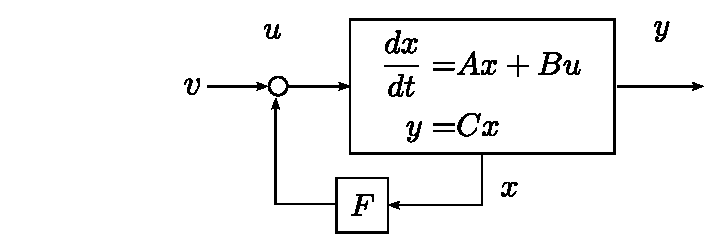
\includegraphics{sfigure/feedback.eps} % scale=100%
  \caption{状態フィードバック}
  \label{fig_state_feedback}
 \end{center}
\end{figure}
%---------------------------------------------------------------------------
\subsection{極配置問題 \label{sec_pole_place}}
%---------------------------------------------------------------------------
フィードバック行列$F$を選ぶことにより，閉ループ系の極を（任意の）指定された値
にする問題を{\bf 極配置(pole assignment)問題}という．

閉ループ系の望ましい極($A+BF$の極)を$p_1, p_2, \cdots, p_n$
とする．極配置問題は，$(A + B F)$の特性多項式$\det (s I - (A + B F))$が
\begin{align}
 \det (s I - (A + B F))
 &= (s - p_1)(s - p_2) \cdots (s - p_n) \nonumber \\
 &\defeq s^n + \mu_{n-1} s^{n-1} + \mu_{n-2} s^{n-2}
  + \cdots + \mu_1 s^1 + \mu_0
\end{align}
となるような$F$を求める問題となる．ここで$\mu_i$が実数となるように$p_i$
が選ばれていると仮定する．これは$p_i = \xi_i + j \eta_i $であり$\eta_i
\neq 0$であるならば$p_j = \xi_i - j \eta_i$も指定された極に含まれてい
るという仮定である．

この問題は{\bf 可制御なシステムについて可解}となることが知られている．

\subsubsection{簡単なシステムの極配置（例）}

例えば，
\begin{equation}
 \frac{d}{dt}
 \left(
 \begin{array}{c}
  x_1 \\
  x_2
 \end{array}
 \right) =
 \left(
 \begin{array}{cc}
  0 & 1\\
  1 & 1
 \end{array}
 \right)
 \left(
 \begin{array}{c}
  x_1 \\
  x_2
 \end{array}
 \right) +
 \left(
 \begin{array}{c}
  0 \\
  1
 \end{array}
 \right) u
\end{equation}
で表されるシステムの極を$-1, -2$とする状態フィードバック$F$を求めてみる．
$u = Fx = (\begin{array}{cc}f_1 & f_2\end{array})x$とすると，
\begin{align}
 \frac{d}{dt}
 \left(
 \begin{array}{c}
  x_1 \\
  x_2
 \end{array}
 \right)
 &=
 \left(
 \begin{array}{cc}
  0 & 1\\
  1 & 1
 \end{array}
 \right)
 \left(
 \begin{array}{c}
  x_1 \\
  x_2
 \end{array}
 \right) +
 \left(
 \begin{array}{c}
  0 \\
  1
 \end{array}
 \right)
 \left(
 \begin{array}{cc}
  f_1 & f_2
 \end{array}
 \right)
 \left(
 \begin{array}{c}
  x_1 \\
  x_2
 \end{array}
 \right)
\nonumber \\
 &=
 \left(
 \begin{array}{cc}
  0 & 1\\
  1 & 1
 \end{array}
 \right)
 \left(
 \begin{array}{c}
  x_1 \\
  x_2
 \end{array}
 \right) +
 \left(
 \begin{array}{cc}
  0   & 0 \\
  f_1 & f_2
 \end{array}
 \right)
 \left(
 \begin{array}{c}
  x_1 \\
  x_2
 \end{array}
 \right)
\nonumber \\
 &=
 \left(
 \begin{array}{cc}
  0 & 1 \\
  1 + f_1 & 1 + f_2
 \end{array}
 \right)
 \left(
 \begin{array}{c}
  x_1 \\
  x_2
 \end{array}
 \right)
\end{align}
となるので，フィードバック系の特性多項式は以下のようになる．
\begin{equation}
 \det(sI - (A + BF))= 
	\det \left (
		\begin{array}{cc}
			s & -1 \\
			-(1+f_1) & s-(1+f_2)
		\end{array}
	\right )
	= s^2 - (1 + f_2) s - (1 + f_1)
\end{equation}
一方，望ましいフィードバック系の特性多項式は極を$-1, -2$とすることから，
\begin{equation}
 (s + 1)(s + 2) = s^2 + 3 s + 2
\end{equation}
である．これらの係数を比較することで，求めるフィードバック行列は
$F = (\begin{array}{cc}f_1 & f_2\end{array}) = 
(\begin{array}{cc}-3 & -4\end{array})$となる．
\\

\noindent
{\bf ＜演習＞極配置} \nopagebreak

次の状態方程式
\begin{align*}
	\frac{d}{dt}
	\left (
	\begin{array}{c}
	 x_1 \\ x_2 
	\end{array}
	\right )
	& = 
	\left (
	\begin{array}{cc}
	 0 & 1 \\
	 0 & -1
	\end{array}
	\right )
	\left (
	\begin{array}{c}
	 x_1 \\ x_2 
	\end{array}
	\right )
	+
	\left (
	\begin{array}{c}
	 0 \\ 1 
	\end{array}
	\right )
	u
\end{align*}
に対して閉ループ系の極が$-4,-5$となるような状態フィードバック
\begin{align*}
	u 
	&=
	\left (
	\begin{array}{cc}
	 f_1 & f_2
	\end{array}
	\right )
	\left (
	\begin{array}{c}
	 x_1 \\ x_2 
	\end{array}
	\right )
\end{align*}
を求めよ．


\subsubsection{1入力可制御正準形で表されたシステムの極配置}

極配置問題は一入力可制御な系に対しては簡単に解ける．ここでは
一入力可制御正準形で表されたシステムの極配置問題の解法を与える．一般の
一入力可制御システムはシステムを可制御正準系に座標変換することにより
この手法を用いて極配置問題を解くことができる．
(可制御正準系でないシステムに対しても，科学技術計算ソフトウェア(MATLAB$^{\tiny \textregistered}$ (http://jp.mathworks.com/)など)の普及により，極配置フィードバックの数値解が容易に得られるようになっている．)


次の可制御正準形で表されたシステムを考える．
\begin{align}
 \frac{d}{dt}
  \left(\begin{array}{c}
         x_1 \\
	 x_2 \\
	 \vdots \\
	 x_{n-1} \\
	 x_n
	\end{array}\right)
  &=
  \left(\begin{array}{ccccc}
     0      & 1      & 0      & \cdots & 0 \\
	 0      & 0      & 1      & \ddots & \vdots \\
	 \vdots & \vdots & \ddots & \ddots & 0 \\
	 0      & 0      & \cdots & 0      & 1 \\
	 -a_0   & -a_1   & \cdots & -a_{n-2} & -a_{n-1}
	\end{array}\right)
  \left(\begin{array}{c}
	 x_1 \\
	 x_2 \\
	 \vdots \\
	 x_{n-1} \\
	 x_n
	\end{array}\right)
  +
  \left(\begin{array}{c}
         0 \\
	 0 \\
	 \vdots \\
	 0 \\
	 1
	\end{array}\right)
  u 
\end{align}
可制御正準形を導入したときに示したように，このシステムの$A$行列の特性多項式は$A$行列の最下列の値を用いて
\begin{equation}
 \det (sI-{A}) = s^n + a_{n-1} s^{n-1} 
  + a_{n-2} s^{n-2} + \cdots + a_1 s + a_0
\end{equation}
と与えられる．

いま，状態フィードバックとして
\begin{align}
 u = F x = 
 (f_1, f_2, \cdots, f_{n-1}, f_{n}) 
 \left(\begin{array}{c}
        x_1 \\
		x_2 \\
		\vdots \\
		x_{n-1} \\
		x_n
       \end{array}\right)
\end{align}
を用いると，状態方程式は
\begin{align}
 \frac{dx}{dt} &= (A+BF)x 
\nonumber \\
 \frac{d}{dt}
  \left(\begin{array}{c}
         x_1 \\
	 x_2 \\
	 \vdots \\
	 x_{n-1} \\
	 x_n
	\end{array}\right)
  &=
  \left(\begin{array}{ccccc}
     0      & 1      & 0      & \cdots & 0 \\
	 0      & 0      & 1      & \ddots & \vdots \\
	 \vdots & \vdots & \ddots & \ddots & 0 \\
	 0      & 0      & \cdots & 0      & 1 \\
	 f_1-a_0   & f_2 -a_1   & \cdots & f_{n-1} -a_{n-2} & f_{n} -a_{n-1}
	\end{array}\right)
  \left(\begin{array}{c}
	 x_1 \\
	 x_2 \\
	 \vdots \\
	 x_{n-1} \\
	 x_n
	\end{array}\right)
\end{align}
となり，その$A+BF$の特性多項式は
\begin{equation}
 \det (sI-{(A+BF)}) = s^n + (a_{n-1}-f_n) s^{n-1} 
  + (a_{n-2}-f_{n-1}) s^{n-2} + \cdots + (a_1-f_2) s + (a_0-f_1)
\label{eq:poleas_cha1}
\end{equation}
となる．一方，システムの望ましいシステムの極($A+BF$の極)を$p_1, p_2, \cdots, p_n$
とすれば$(A + B F)$の特性多項式$\det (s I - A - B F)$は$p_i$から導出される$\mu_i$を用いて
\begin{align}
 \det (s I - A - B F)
 &= (s - p_1)(s - p_2) \cdots (s - p_n) \nonumber \\
 &\defeq s^n + \mu_{n-1} s^{n-1} + \mu_{n-2} s^{n-2}
  + \cdots + \mu_1 s^1 + \mu_0
\label{eq:poleas_cha2}
\end{align}
とならなければならない．(\ref{eq:poleas_cha1})と(\ref{eq:poleas_cha2})が等しくなるためにはおのおのの係数が等しい必要がある．つまり，
\begin{align}
 \mu_0 & = a_0-f_1
\nonumber\\
 \mu_{1} & = a_1-f_2
\nonumber\\
 \vdots
\\
 \mu_{n-2} & = a_{n-2}-f_{n-1}
\nonumber\\
　\mu_{n-1} & = a_{n-1}-f_n
\nonumber
\end{align}
である必要がある．これを$f_i$についてとけば
\begin{align}
 f_1 & = a_0-\mu_0
\nonumber\\
 f_2 & = a_1-\mu_{1}
\nonumber\\
 \vdots
\\
 f_{n-1} & = a_{n-2}-\mu_{n-2}
\nonumber\\
　f_n& = a_{n-1}-\mu_{n-1} 
\nonumber
\end{align}
とすれば極配置問題が解けたことになる．これを$F$行列で表せば
\begin{equation}
 {F} = \left(\begin{array}{cccc}
	          a_0-\mu_0, & a_1-\mu_1, & \cdots, & a_{n-1}-\mu_{n-1}
		 \end{array}\right)
\end{equation}
となる．

ここまでの議論を用いれば状態方程式を可制御正準形に座標変換できれば極配置問題が解けることがわかる．可制御正準形への変換についてはここでは扱わない．



%---------------------------------------------------------------------------
\subsection{極と応答}
%---------------------------------------------------------------------------
システムの極と応答がどのような関係になっているかについて簡単に考察してみ
よう．簡単のために複素係数を持つ1次のシステムを考える．
\begin{align}
 \dot{x} &= \lambda \ x \nonumber \\
         &= (\alpha + j \beta) x
\end{align}
このシステムの極は明らかに$\alpha + j\beta$であるから，極の実部は$\alpha$，
極の虚部は$\beta$である．また，この微分方程式を解けばシステムの応答は
\begin{align}
 x(t) &= e^{(\alpha + j \beta)t} x(0) \nonumber \\
      &= e^{\alpha t}e^{j \beta t} x(0)
\end{align}
となることが簡単にわかる．さらに
\begin{equation}
 e^{j \beta t} = \cos(\beta t) + j \sin(\beta t)
\end{equation}
であることを用いれば
\begin{align}
 x(t) &= e^{\alpha t} \{ \cos(\beta t) + j \sin(\beta t) \}x(0) \nonumber \\
      &= e^{\alpha t} \cos(\beta t) x(0) + j e^{\alpha t} \sin(\beta t)x(0)
\end{align}
となる．

さて，極とシステムの応答の関係を直感的に理解するためには，$x(0)=1$の場合の応
答の{実部}，つまり
\begin{equation}
 x(t) = e^{\alpha t} \cos(\beta t)
\end{equation}
について検討すれば十分である．
この応答は$e^{\alpha t}$と$\cos(\beta t)$を乗じたものである．

さて，それでは$\alpha$と$\beta$の大きさによるシステムの応答の違いはどうだろ
うか．Fig.\ref{fig_pole12}は$e^{\alpha t}$と$\cos(\beta t)$をそれぞれ
$\alpha=0.5, -1, -5$と$\beta=2, 10$について描いたものである．ここで
\begin{itemize}
 \item $\alpha$は極の実部に，$\beta$は極の虚部に対応している．
 \item $\alpha>0$のときは$e^{\alpha t}$は発散，$\alpha<0$のときは
       $e^{\alpha t}$は$0$に収束する．
 \item $\alpha$が小さいほど(負で絶対値が大きいほど)$e^{\alpha t}$は速
       く０に収束する．
 \item $\beta$が大きいほど$\cos(\beta t)$の振動が速くなる．
 \item $e^{\alpha t}$と$ \cos(\beta t)$を乗じたものがシステムの応答になる．
\end{itemize}
ことに注意すれば以下の考察はほとんど自明であろう．

Fig.\ref{fig_pole34}は$\beta = 10$と固定し，$\alpha = 0.5, -1$と変化させ
た場合の応答の変化である．
明らかに$\alpha > 0$のときは応答が発散し，$\alpha < 0$のときは安定
となることがわかる．これは
\begin{quote}
 (1) 極の実部が負のときシステムは安定(正のときは不安定)である
\end{quote}
ことを示している．

Fig.\ref{fig_pole56}は$\beta = 2$と固定して$\alpha = -1, -5$と変化さ
せた場合の応答の変化である．
明らかに$e^{\alpha t}$の収束の速さに引きずられて$\alpha=-5$の時
の方が収束が速くなっている．これは
\begin{quote}
 (2) 極の実部が小さいほど(負で絶対値が大きいほど)応答が速く0に収束する
\end{quote}
ことを示している． 

\begin{figure}[t!]
 \begin{minipage}{0.5\textwidth}
  \begin{center}
   \input{figure/fig1.pstex_t} % scale=60%
   (a) $e^{\alpha t}$
  \end{center}
 \end{minipage}%
 \begin{minipage}{0.5\textwidth}
  \begin{center}
   \input{figure/fig2.pstex_t} % scale=60%
   (b) $\cos \beta t$
  \end{center}
 \end{minipage}
 \caption{極と応答1}
 \label{fig_pole12}
\end{figure}

\begin{figure}[t!]
 \begin{minipage}{0.5\textwidth}
  \begin{center}
   \input{figure/fig3a.pstex_t} % scale=60%
   (a) $\alpha = 0.5$
  \end{center}
 \end{minipage}%
 \begin{minipage}{0.5\textwidth}
  \begin{center}
   \input{figure/fig3b.pstex_t} % scale=60%
   (b) $\alpha = -1$
  \end{center}
 \end{minipage}
 \caption{極と応答2 $(\beta = 10)$}
 \label{fig_pole34}
\end{figure}

\begin{figure}[t!]
 \begin{minipage}{0.5\textwidth}
  \begin{center}
   \input{figure/fig4a.pstex_t} % scale=60%
   (a) $\alpha = -1$
  \end{center}
 \end{minipage}%
 \begin{minipage}{0.5\textwidth}
  \begin{center}
   \input{figure/fig4b.pstex_t} % scale=60%
   (b) $\alpha = -5$
  \end{center}
 \end{minipage}
 \caption{極と応答3 $(\beta = 2)$}
 \label{fig_pole56}
\end{figure}

Fig.\ref{fig_pole78}は$\alpha = -1$と固定して$\beta = 2, 10$と変化させ
た場合の応答の変化である．
基本的な原点への収束の速さは$e^{\alpha t}$が等しいので同じである
が，$\beta$が大きい方が応答が振動的になることがわかる．これは
\begin{quote}
(3) 極の虚部が大きくなるほど応答が振動的になる
\end{quote}
ことを示している． 

Fig.\ref{fig_pole910}は$\alpha = -1, \beta = 2$と$\alpha = -5, \beta = 10$の
場合の応答を示している．
これらの応答の原点への収束はもちろん$\alpha = -5$の方が速いが，
オーバーシュートはほとんど同じである．
つまり，振動性がほとんど同じであることがわかる．これは
\begin{quote}
 (4) システムの振動性が極の実部と虚部の比で決定される 
\end{quote}
ことを示している．

\begin{figure}[t!]
 \begin{minipage}{0.5\textwidth}
  \begin{center}
   \input{figure/fig5a.pstex_t} % scale=60%
   (a) $\beta = 2$
  \end{center}
 \end{minipage}%
 \begin{minipage}{0.5\textwidth}
  \begin{center}
   \input{figure/fig5b.pstex_t} % scale=60%
   (b) $\beta = 10$
  \end{center}
 \end{minipage}
 \caption{極と応答4 ($\alpha = -1$)}
 \label{fig_pole78}
\end{figure}

\begin{figure}[t!]
 \begin{minipage}{0.5\textwidth}
  \begin{center}
   \input{figure/fig6a.pstex_t} % scale=60%
   (a) $\alpha = -1, \beta = 2$
  \end{center}
 \end{minipage}%
 \begin{minipage}{0.5\textwidth}
  \begin{center}
   \input{figure/fig6b.pstex_t} % scale=60%
   (b) $\alpha = -5, \beta = 10$
  \end{center}
 \end{minipage}
 \caption{極と応答5}
 \label{fig_pole910}
\end{figure}

\begin{figure}[h]
 \begin{center}
  \input{figure/pole.pstex_t} % scale = 100%
  \caption{望ましい極配置}
  \label{fig_pole}
 \end{center}
\end{figure}

さらに，極配置法を用いて制御系を設計する場合には
\begin{quote}
 (5) 応答を速くする(閉ループ系の極の実部を小さくする)と入力が大きくなる 
\end{quote}
ことに注意して極端に応答を速くしないことが必要となる．

これらを念頭に置いて，極配置を行うときはFig.\ref{fig_pole}のような範囲に
極を配置することが良いとされている．

\pagebreak

%---------------------------------------------------------------------------
\subsection{最適制御 \label{sec_opt}}
%---------------------------------------------------------------------------
前節では安定化フィードバックを極配置により求める方法を示した．しかしこの
方法では多入力系の場合にはフィードバックが一意に決まらないなど不都合が生
じる場合がある．
例えば，
\[
 \frac{d}{dt}
 \left(
 \begin{array}{c}
  x_1 \\
  x_2
 \end{array}
 \right) =
 \left(
 \begin{array}{cc}
  1 & 0 \\
  0 & 1
 \end{array}
 \right) 
 \left(
 \begin{array}{c}
  x_1 \\
  x_2
 \end{array}
 \right) +
 \left(
 \begin{array}{cc}
  1 & 0 \\
  0 & 1
 \end{array}
 \right)
 \left(
 \begin{array}{c}
  u_1 \\
  u_2
 \end{array}
 \right)
\]
で表されるシステムに対して，
\begin{align*}
 u &=
 \left(
 \begin{array}{cc}
  -2 & 0 \\
  0 & -3
 \end{array}
 \right)
 \left(
 \begin{array}{c}
  x_1 \\
  x_2
 \end{array}
 \right)のとき，\\
 & \quad
 A+BF = 
 \left(
 \begin{array}{cc}
  -1 & 0 \\
  0 & -2
 \end{array}
 \right), \ \ 
 \det(sI - (A + BF)) =
 \det\left(
 \begin{array}{cc}
  s+1 & 0 \\
  0 & s+2
 \end{array}
 \right)
 = s^2 + 3s + 2 \\[5mm]
 u &=
 \left(
 \begin{array}{cc}
  -3 & 0 \\
  0 & -2
 \end{array}
 \right)
 \left(
 \begin{array}{c}
  x_1 \\
  x_2
 \end{array}
 \right)のとき，\\
 & \quad
 A+BF = 
 \left(
 \begin{array}{cc}
  -2 & 0 \\
  0 & -1
 \end{array}
 \right), \ \ 
 \det(sI - (A + BF)) =
 \det\left(
 \begin{array}{cc}
  s+2 & 0 \\
  0 & s+1
 \end{array}
 \right)
 = s^2 + 3s + 2 \\[5mm]
 u &=
 \left(
 \begin{array}{cc}
  -1 & 1 \\
  -2 & -4
 \end{array}
 \right)
 \left(
 \begin{array}{c}
  x_1 \\
  x_2
 \end{array}
 \right)のとき，\\
 & \quad
 A+BF = 
 \left(
 \begin{array}{cc}
  0 & 1 \\
  -2 & -3
 \end{array}
 \right), \ \ 
 \det(sI - (A + BF)) =
 \det\left(
 \begin{array}{cc}
  s & -1 \\
  2 & s+3
 \end{array}
 \right)
 = s^2 + 3s + 2
\end{align*}
のように，異なるフィードバック行列に対し，フィードバック系の極が
全て$-1, -2$となる．つまり，極を指定してもどのフィードバック行列を用いれ
ばいいのかわからないことになる．

これに対して安定化フィードバックを次の２次形式評価関数を
最小にするように選ぶ方法(最適フィードバック)がある．
\begin{equation}
 J = \int_{0}^{\infty} (x^T Q x + u^T R u) dt
\label{eqn:P-index}
\end{equation}
ここで$Q$は半正定($Q = H^T H$で表わされる)，$R$は正定($R = L^T L$, ($L$
は正則行列)で表わせる)とする．この$J$を最小にするフィードバックは，$P$を
Riccati方程式
\begin{equation}
 A^T P + P A - P B R^{-1} B^T P + Q = 0
\end{equation}
の正定解として
\begin{equation}
   u = - R^{-1} B^T P x \defeq Fx
\end{equation}
で表わされることが知られている．さらに$(H,A)$が可観測であれば閉ループ系
が安定になる．

$Q(=H^T H)$と$R(=L^T L)$は以下のように選ばれることが多い．
\begin{equation}
 H = \left(\begin{array}{cccc}
            h_1    & 0   & \cdots & 0 \\
	    0      & h_2 &        & 0 \\
	    \vdots &     & \ddots & \\
	    0      & 0   &        & h_n 
	   \end{array}\right)
 , \quad
 L = \left(\begin{array} {cccc}
            l_1    & 0   & \cdots & 0 \\
	    0      & l_2 &        & 0 \\
	    \vdots &     & \ddots & \\
	    0      & 0   &        & l_m 
	   \end{array}\right)
\end{equation}
($h_i>0$, $l_j>0$). このとき，$x = (x_1, x_2, \cdots, x_n)^T$, $u = (u_1, u_2, \cdots, u_m)^T$であることを用いて評価関数を書き下せば，
\begin{align}
 J
 &= \int_{0}^{\infty} (x^T Q x + u^T R u) dt \nonumber \\
 &= \int_{0}^{\infty} (x^T H^TH x + u^T L^TL u) dt \nonumber \\
 &= \int_{0}^{\infty} ((Hx)^TH x + (Lu)^TL u) dt \nonumber \\
 &= \int_{0}^{\infty}
    \left\{
    \left(
    \begin{array}{cccc}
     h_1x_1 & h_2x_2 & \cdots & h_nx_n
    \end{array}
    \right)
    \left(
    \begin{array}{c}
     h_1x_1 \\
     h_2x_2 \\
     \vdots \\
     h_nx_n
    \end{array}
    \right) +
    \left(
    \begin{array}{cccc}
     l_1u_1 & l_2u_2 & \cdots & l_mu_m
    \end{array}
    \right)
    \left(
    \begin{array}{c}
     l_1u_1 \\
     l_2u_2 \\
     \vdots \\
     l_mu_m
    \end{array}
    \right)
    \right\}dt \nonumber \\
 &= \int_0^{\infty} (h_1^2 x_1^2 + h_2^2 x_2^2 + \cdots +
     h_n^2 x_n^2 + l_1^2 u_1^2 + \cdots + l_m^2 u_m^2)dt
\label{eqn:P-index2}
\end{align}
となる．この評価関数の意味について考えてみよう．

\begin{figure}
 \begin{center}
  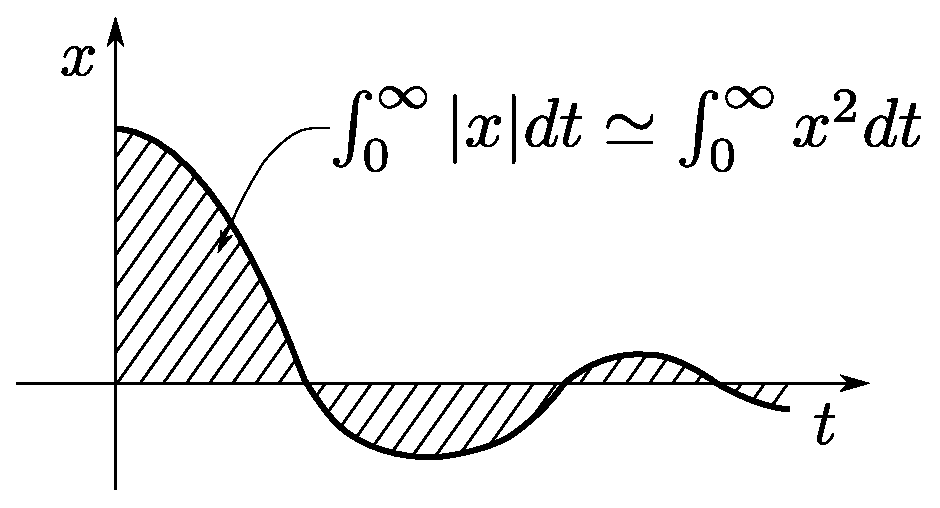
\includegraphics[width=0.6\linewidth]{sfigure/optimal.eps} % scale = 100%
  \caption{評価関数のイメージ}
  \label{fig_J}
 \end{center}
\end{figure}


ここでは，評価関数(\ref{eqn:P-index2})の第１項として以下の部分を考えよう．
\begin{align}
	J' &= \int_0^\infty x_1^2 dt
\end{align}
これは$x$の2乗積分である．2乗積分を図に表すのは難しいので，これと同じようなものとして次の絶対値積分を考える．
\begin{align}
	J'' &= \int_0^\infty | x_1 | \ dt
\end{align}
これはFig~\ref{fig_J}の斜線部分の面積に相当する．評価関数$J''$を最小化するということはこの斜線の面積を最小化する．つまり，$x$を速く$0$に収束させるということに相当することがわかる．$J'$の最小化も同等の効果がある．

このように評価関数(\ref{eqn:P-index2})の$x_i$に関する項を最小化するということは，$x_i$を速く$0$に収束させるという問題設定と考えることができる．

一方，同様に評価関数(\ref{eqn:P-index2})の$u_j$に関する項を最小化するということは入力を極力使わないということに対応する．

このように，評価関数(\ref{eqn:P-index2})を最小化するということは，できるだけ入力$u$を用いずに，できるだけ速く$x$を$0$に収束させたいという問題設定と考えることができる．それぞれの項の重みづけが$h_i$, $l_j$ ($Q$, $R$)ということになる．

実際の設計時における$Q$, $R$は試行錯誤で選ぶこととなるが，次のような方針で状態フィードバックを設計することにより，望ましい応答を容易に得ることができる．

いま，ある$H$, $L$に対する閉ループ系の応答を調べたところ
$x_1$が大きくふれすぎることがわかったとしよう．
このときは$h_1$を大きくして再設計すれば$J$に対する$x_1$の寄与が大きくな
るため，$J$を小さくするためには$x_1$を小さくしなければならなくなり
結果的に$x_1$をおさえる制御系が設計できる．
同様に$x_i$と$u_j$の挙動が激しい(大きく動く)ならば$h_i$と$l_j$を
大きくすれば$x_i$, $u_j$の動きが抑えられる．

通常，$h_i^2$, $l_j^2$の増減は$10$倍，$1/10$を目安にすることが多い．つまり，$1$の次は$10$, その次は$100$であり，$1$の前は$1/10$として調整することが多い．
\\

\noindent
{\bf ＜演習＞最適制御：不安定極} \nopagebreak

次のシステムと評価関数に対する最適制御を求めよ．
\begin{align*}
	\frac{dx}{dt} & = 1 \cdot x + 1 \cdot u \ \ \ \ \ \ \ \ \ \ \ \ A=1,B=1\\
	J & = \int_0^{\infty} x^2 + r u^2 dt \ \ \ \ \ \ \ \ Q=1,R=r
\end{align*}
また，$r\rightarrow 0$と$r\rightarrow \infty$の場合の入力とフィードバック系の極を求めよ．
\\

\noindent
{\bf ＜演習＞最適制御：安定極} \nopagebreak

次のシステムと評価関数に対する最適制御を求めよ．
\begin{align*}
	\frac{dx}{dt} & = \underline{-1} \cdot x + 1 \cdot u \ \ \ \ \ \ \ \ \ \ \ \ A=\underline{-1},B=1\\
	J & = \int_0^{\infty} x^2 + r u^2 dt \ \ \ \ \ \ \ \ Q=1,R=r
\end{align*}
また，$r\rightarrow 0$と$r\rightarrow \infty$の場合の入力とフィードバック系の極を求めよ．

\subsubsection{Riccati方程式の解法}

Riccati方程式の解法としては，数値的に安定な以下の有本-Potterの方法がよく用
いられる．まず行列$\Phi$を次のように定義する．
\begin{align}
 \Phi = \left(\begin{array}{cc}
	       A  & - B R^{-1} B^T \\
	       -Q & - A^T
	      \end{array}\right)
\end{align}
この$\Phi$の固有値のうち実部が負のものが$n$個あることが分かっている．これらの固有値を$\lambda_i$, $i=1,2,\cdots,n$とし，これに対応する固有ベクトルを$w_1, w_2, \cdots, w_n$する．この固有ベクトルを次のように分解しておく．
\begin{align}
 w_i = \left(\begin{array}{c}
	      \xi_i \\
	      \eta_i
	     \end{array}\right), \hspace{1cm} \xi_i \in {\mathbb R}^n, \ \eta_i \in {\mathbb R}^n
\end{align}
このとき
\begin{align}
	P = Y X^{-1}, \ \ \ 
	X = (\xi_1, \xi_2, \cdots, \xi_n), \ \ \ 
	Y = (\eta_1, \eta_2, \cdots, \eta_n)
\end{align}
と選べば$P$は正定かつRiccati方程式を満たすことが知られている．

このほかにLMI(線形行列不等式)\cite{ebihara}を用いた方法などがある．

科学技術計算ソフトウェア(MATLAB$^{\tiny \textregistered}$ (http://jp.mathworks.com/)など)の普及により，最適フィードバックの数値解が容易に得られるようになっている．


%Riccati方程式の解法と最適制御の性質については後に詳解する．
%---------------------------------------------------------------------------
\subsection{リアプノフ関数とシステムの安定性}
%---------------------------------------------------------------------------
システムの安定性を保証する，極を調べる以外の方法として，リアプノフ関数を用いた方法について簡単に述べておこう．

正則行列$T$(と$P=T^T T$)を用いて
\begin{equation}
 V(x) = x^T T^T T x = x^T P x
\end{equation}
なるスカラー関数を考えよう．これは座標変換された状態ベクトル
\begin{equation}
 \bar{x} = T x
\end{equation}
に対して
\begin{equation}
 V(x) = \bar{x}^T \bar{x} = | \bar{x} | ^2
\end{equation}
を考えていることに相当するので，$V(x) \geq 0$でかつ$V(x) = 0$となるのは$x=0$
, ($\bar{x} = 0 $)のみである．このような$V(x)$のことを{\bf 正定関数(Positive Definite Function)}，$P$のことを
{\bf 正定行列(Positive Definite Matrix)}と呼ぶ．

さて，いまこの関数$V(x)$を時間微分したものが
\begin{equation}
 \frac{d V}{d t} < 0, \quad x \neq 0
  \label{lyapunov_1}
\end{equation}
と表されたとすると，これは$x \neq 0$である限り$V$が時間に対して単調減少する
ことを示し，最終的に$ V \rightarrow 0$ ($t \rightarrow \infty$)と
なること，つまり，$x(t) \rightarrow 0$となること(システムが安定であるこ
と)を示している．
このような関数$V(x)$は{\bf リアプノフ関数(Lyapunov Function)}と呼ばれ，システムの安定性
を証明するときによく用いられる．
リアプノフ関数のイメージをFig.\ref{fig:lyapunov}に示す．

\begin{figure}[htbp]
 \begin{center}
  \input{figure/lyapunov.pstex_t} % scale = 100%
  \caption{リアプノフ関数のイメージ}
  \label{fig:lyapunov}
 \end{center}
\end{figure}


これを用いて最適制御の安定性を証明してみよう．最適フィードバックがRiccati方
程式の正定解$P$を用いて$u = -R^{-1} B^T P x$となることから，閉ループ系は
\begin{align}
 \frac{dx}{dt} &= Ax + B u \nonumber \\
               &= (A - B R^{-1} B^T P)x
 \label{LQ_opt}
\end{align}
となる．いまリアプノフ関数の候補としてRiccati方程式の正定解$P$を用いて$V(x) 
= x^T P x$を考える．この$V(x)$の微分は(\ref{LQ_opt})と$P^T = P$である事実を
用いて
\begin{align}
 \frac{d V}{dt}
  &= \frac{d x^T}{dt} P x + x^T P \frac{dx}{dt} \nonumber \\
 &= [(A - B R^{-1} B^T P)x]^T Px + x^T P (A - B R^{-1} B^T P)x \nonumber \\
 &= x^T (A^T - P B R^{-1} B^T ) P x + x^T P (A - B R^{-1} B^T P)x \nonumber \\
 &= x^T (A^T P + P A - 2P B R^{-1} B^T P) x
\end{align}
と計算できる．さらにRiccati方程式を変形すると
\begin{equation}
 A^T P + P A = P B R^{-1} B^T P - Q
\end{equation}
となることから，これを$A^T P + P A$の部分に代入すれば
\begin{equation}
 \frac{dV}{dt} = - x^T (P B R^{-1} B^T P + Q) x
\end{equation}
であることがわかる．ここで$R = L^T L$, $Q = H^T H$と表され，かつ$L, H$が正
則のとき，右辺は
\begin{align}
 - x^T (P B R^{-1} B^T P + Q) x 
  &= - x^T (L^{-T} B^T P)^T (L^{-T} B^T P) x -   x^T H^T H x \nonumber \\
  &= - |(L^{-T} B^T P) x|^2 -  |H x|^2 \nonumber \\
 &< 0, \quad (x \neq 0)
\end{align}
と表わされ，システムの安定性が証明される．
$H$が正則でない場合にはもう少し精密な議論が必要であるが，ここでは省略す
る．

%---------------------------------------------------------------------------
\subsection{サーボ系}\label{subsec:servo}
%---------------------------------------------------------------------------
出力$y$をある目標値$r$に追従させたいことがよくある．この目的のためにつく
られたフィードバック系をサーボ系と呼ぶ．ここでは特にステップ目標値($r$が一定
値)の場合について扱う．古典理論でもよく知られているように，定常偏差が零に
なるようにするためには，
Fig.\ref{fig_servo0} のように (1)~コントローラが積分器を持ち，(2)~閉ループ系が安定であれば良いことが分かっている（解釈は後述）．
そこでこの知識をもとにサーボ系を設計する方法を示す．
\begin{figure}[t]
 \begin{center}
  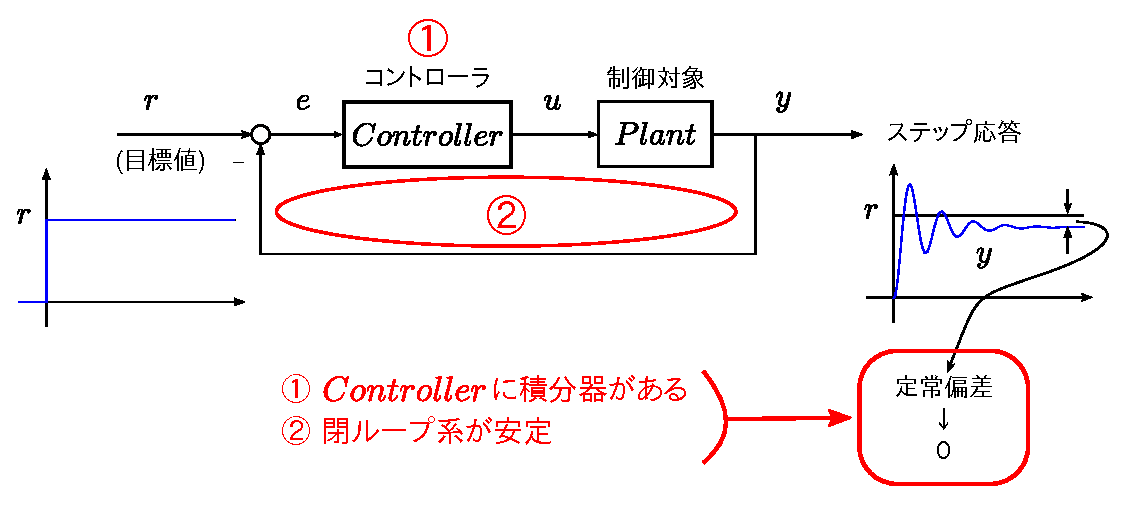
\includegraphics[width=0.8\linewidth]{sfigure/stdError.eps}
  \caption{古典制御理論におけるサーボ系}
  \label{fig_servo0}
 \end{center}
\end{figure}

ここではシステム(\ref{state_eq})(\ref{output_eq})において$D=0$とした以
下の系を考える．
\begin{align}
 \frac{dx}{dt} &= A x + B u \label{st_proper_state_eq} \\
 y             &= C x \label{st_proper_output_eq}
\end{align}
さらに$y \in \mathbb{R}^m$であり，入力と出力の次数が等しいとする．

追従誤差を$e=r-y$として次式で積分器を導入する．
\begin{equation}
 \eta = \int_0^t e \ d\tau
\end{equation}
両辺を$t$ で微分すると，
\begin{equation}
 \frac{d \eta}{dt} = e= r - y = r - Cx
\end{equation}
をとなり，積分器を状態方程式（微分方程式）で表すことができる．
この積分器とシステム(\ref{st_proper_state_eq})
(\ref{st_proper_output_eq})を合わしたFig.~\ref{fig_servo1}のシステム(拡大系)は
\begin{align}
 \frac{d}{dt}
  \left(\begin{array}{c}
         x \\
	 \eta
	\end{array}\right)
  &=
  \left(\begin{array}{cc}
         A  & 0 \\
	 -C & 0
	\end{array}\right)
  \left(\begin{array}{c}
         x \\
	 \eta
	\end{array}\right)
  +
  \left(\begin{array}{c}
         B \\
	 0
	\end{array}\right)
  u +
  \left(\begin{array}{c}
         0 \\
	 I
	\end{array}\right) 
  r \\
 y &=
  \left(\begin{array}{cc}
         C & 0 
	\end{array}\right)
  \left(\begin{array}{c}
         x \\
	 \eta
	\end{array}\right)
\end{align}
となる．

このシステムは$(A,B)$可制御かつ
\begin{equation}
   \rank \left(\begin{array}{cc}
	        A & B \\
		C & 0
	       \end{array}\right)
   = n + m
\end{equation}
のとき安定化できることが知られている．
\begin{figure}[t]
 \begin{center}
  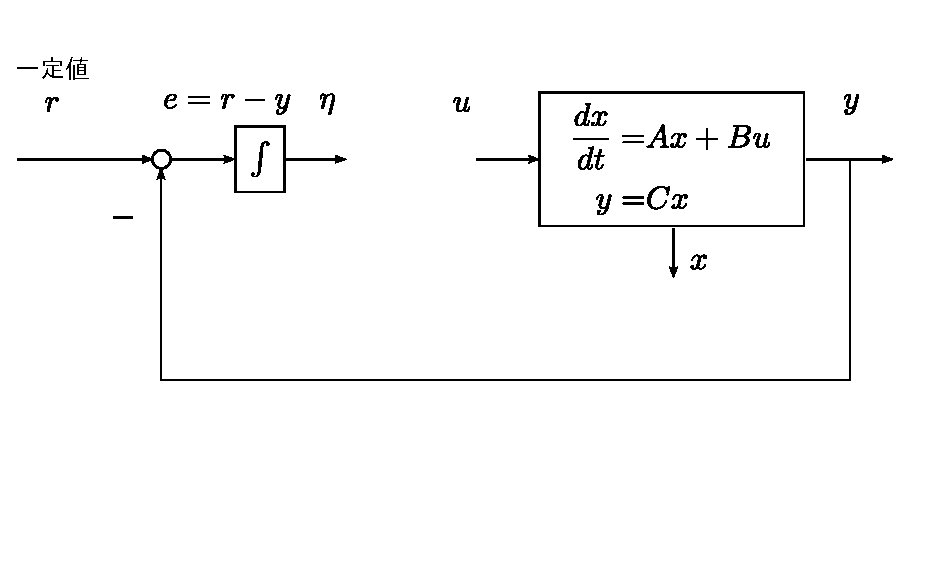
\includegraphics[width=0.7\linewidth]{sfigure/servo1.eps}
  \caption{積分器を含む拡大系}
  \label{fig_servo1} 
 \end{center}
\end{figure}


さて，この拡大システムを安定化さ
せる状態フィードバックは極配置法や最適制御法で求めることができる．状態フィードバックは
\begin{equation}
 u = \left(\begin{array}{cc}
            F & K 
	   \end{array}\right)
 \left(\begin{array}{c}
        x \\
	\eta
       \end{array}\right)
   = F x + K \eta
\end{equation}
であり，ブロック線図で表せばFig.~\ref{fig_servo2}となる．このシステムは (1)~コントローラに積分器を含み，(2)~閉ループ系が安定，であることから，ステップ目標値（一定目標値）$r$に対して出力$y$が定常偏差を持たずに追従するサーボ系となる．

\begin{figure}
 \begin{center}
  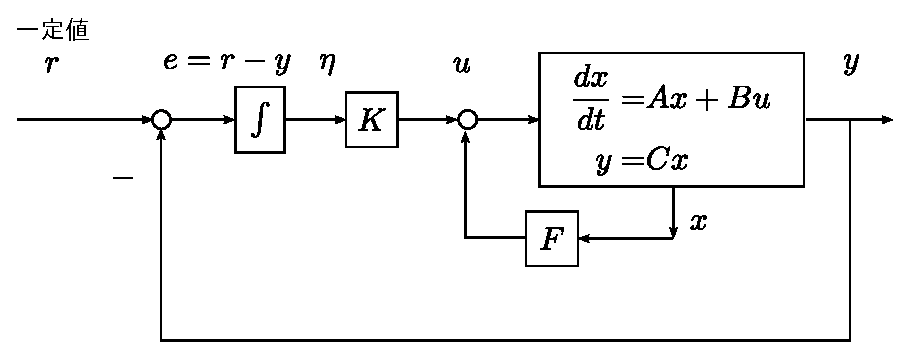
\includegraphics[width=0.7\linewidth]{sfigure/servo2.eps}
  \caption{サーボ系}
  \label{fig_servo2}
 \end{center}
\end{figure}

それでは，なぜ，定常偏差が$0$となるかについて考察しよう．
閉ループ系は
\begin{align}
 \frac{d}{dt}
  \left(\begin{array}{c}
         x \\
	 \eta
	\end{array}\right)
  &=
  \left(\begin{array}{cc}
         A + B F & B K \\
	 - C     & 0
	\end{array}\right)
  \left(\begin{array}{c}
         x \\
	 \eta
	\end{array}\right)
  +
  \left(\begin{array}{c}
         0 \\
	 I
	\end{array}\right) 
  r \\
 y &=
  \left(\begin{array}{cc}
         C & 0 
	\end{array}\right)
  \left(\begin{array}{c}
         x \\
	 \eta
	\end{array}\right)
\end{align}
となる．システムは安定であるから$r$を一定値とすると，$t \rightarrow \infty
$で状態$x$と積分器の状態$\eta$はある値$x_{\infty}$と$\eta_{\infty}$に収
束することを示すことができる（閉ループ系が安定であるから，一定目標値$r$が入ったとしても，システムが振動したり，発散しないことは容易に推測できる）．よって出力$y$も$y_{\infty} = C x_{\infty}$に収束する．$t
\rightarrow \infty $において$\eta$が収束することから
\begin{equation}
 \lim_{t \rightarrow \infty} \frac{d \eta}{dt} = 0
\end{equation}
でなければならない．これは
\begin{equation}
 \lim_{t \rightarrow \infty} \frac{d \eta}{dt}
  = r - y_{\infty} = 0
\end{equation}
であることを示している．よって
\begin{equation}
   \lim_{t \rightarrow \infty} y(t) = y_\infty= r
\end{equation}
つまり，定常偏差が零となる．
\\

\noindent
{\bf ＜演習＞サーボ系} \nopagebreak

次のシステムに対して，一定目標値$r$に対して定常偏差なく追従するコントローラを設計せよ．ただし，閉ループ系のすべての極を$-1$とせよ．
\begin{align*}
	\frac{dx}{dt} &= 1 \cdot x + 1 \cdot u, \hspace{0cm} &A=1,\  B=1
\\
	y &= 1 \cdot x , &C=1, \ D=0
\end{align*}

\subsubsection{内部モデル原理}

ここではステップ目標値に定常偏差なく追従する制御系を設計した．古典制御理論によればランプ目標値($r(t)=t$)に定常偏差なく追従するためには一巡伝達関数が$\frac{1}{s^2}$を，一定加速度目標値($r(t)=\frac{t^2}{2}$）に定常偏差なく追従するためには一巡伝達関数が$\frac{1}{s^3}$を含んでいればよいことが分かっている．これはステップ目標値($r(t)=1$)のラプラス変換は$\frac{1}{s}$,ランプ目標値は$\frac{1}{s^2}$，一定加速度目標値は$\frac{1}{s^3}$であることを考えれば，目標値のラプラス変換と同じ伝達関数を一巡伝達関数に含んでいれば定常偏差なく追従できることを示している．これは{\bf 内部モデル原理(internal model principle)}と言って，例えば同様に$r(t)= \sin \omega t$に追従するためには$\sin \omega t$のラプラス変換である$\frac{\omega}{s^2 + \omega^2}$を一巡伝達関数が含んでいれば定常偏差なく追従できることが知られている．それぞれの伝達関数の状態方程式表現は
\begin{align}
\frac{1}{s^2}: & \hspace*{3mm}
 \frac{d}{dt}
  \left(\begin{array}{c}
         \eta_1 \\
	 \eta_2
	\end{array}\right)
  =
  \left(\begin{array}{cc}
         0 & 1 \\
	 0 & 0
	\end{array}\right)
  \left(\begin{array}{c}
         \eta_1 \\
	 \eta_2
	\end{array}\right)
  +
  \left(\begin{array}{c}
         0 \\
	 1
	\end{array}\right)
  u 
  , \hspace{1.5cm}
  y =
  \left(\begin{array}{cc}
         1 & 0 
	\end{array}\right)
  \left(\begin{array}{c}
         \eta_1 \\
	 \eta_2
	\end{array}\right)
\\		
\frac{1}{s^3}: &  \hspace*{3mm}
 \frac{d}{dt}
  \left(\begin{array}{c}
         \eta_1 \\
         \eta_2 \\
	 \eta_3
	\end{array}\right)
  =
  \left(\begin{array}{ccc}
         0 & 1 & 0\\
	 0 & 0 & 1\\
	 0 & 0 & 0
	\end{array}\right)
  \left(\begin{array}{c}
         \eta_1 \\
         \eta_2 \\
	 \eta_3
	\end{array}\right)
  +
  \left(\begin{array}{c}
         0 \\
         0 \\
	 1
	\end{array}\right)
  u 
  , \hspace{0.8cm}
  y =
  \left(\begin{array}{ccc}
         1 & 0 & 0
	\end{array}\right)
  \left(\begin{array}{c}
         \eta_1 \\
         \eta_2 \\
	 \eta_3
	\end{array}\right)
\\
\frac{\omega}{s^2+\omega^2}: & \hspace*{3mm}
 \frac{d}{dt}
  \left(\begin{array}{c}
         \eta_1 \\
	 \eta_2
	\end{array}\right)
  =
  \left(\begin{array}{cc}
         0 & \omega \\
	 -\omega & 0
	\end{array}\right)
  \left(\begin{array}{c}
         \eta_1 \\
	 \eta_2
	\end{array}\right)
  +
  \left(\begin{array}{c}
         0 \\
	 1
	\end{array}\right)
  u 
  , \hspace{1.3cm}
  y =
  \left(\begin{array}{cc}
         1 & 0 
	\end{array}\right)
  \left(\begin{array}{c}
         \eta_1 \\
	 \eta_2
	\end{array}\right)
\end{align}
であることから，これらの状態方程式部分を用いて拡大系を構成し，安定化すればこれらの目標値に対して定常偏差なく追従する制御系が設計できる（状態フィードバックによる安定化を行うため，出力方程式部分は無視してよい）．


\subsubsection{拡大系の可制御性の例題}

ここでは拡大系が可制御となるための条件
\begin{equation}
   \rank \left(\begin{array}{cc}
	        A & B \\
		C & 0
	       \end{array}\right)
   = n + m
\end{equation}
について考える．\\

\noindent
\underline{拡大系が可制御となる例}\nopagebreak

次のシステムを考える．
\begin{align}
 \frac{d}{dt}
 \left(
 \begin{array}{c}
  x_1 \\
  x_2
 \end{array}
 \right) &=
 \left(
 \begin{array}{cc}
  0 & 1 \\
  1 & 2 \\
 \end{array}
 \right)
 \left(
 \begin{array}{c}
  x_1 \\
  x_2
 \end{array}
 \right) +
 \left(
 \begin{array}{c}
  0 \\
  1
 \end{array}
 \right) u \\
 y &= 
 \left(
 \begin{array}{cc}
  1 & 0
 \end{array}
 \right)
 \left(
 \begin{array}{c}
  x_1 \\
  x_2
 \end{array}
 \right)
\end{align}
このシステムに積分器
\begin{align}
 \frac{d\eta}{dt} &= r - y \\
 &= r - Cx \\
 &= r - \left(\begin{array}{cc}1 & 0 \end{array}\right)x
\end{align}
を導入して拡大系を構成すると，
\begin{align}
 \frac{d}{dt}
 \left(
 \begin{array}{c}
  x_1 \\
  x_2 \\
  \eta
 \end{array}
 \right) &=
 \left(
 \begin{array}{ccc}
  0 & 1 & 0 \\
  1 & 2 & 0 \\
  -1 & 0 & 0 \\
 \end{array}
 \right)
 \left(
 \begin{array}{c}
  x_1 \\
  x_2 \\
  \eta
 \end{array}
 \right) +
 \left(
 \begin{array}{c}
  0 \\
  1 \\
  0
 \end{array}
 \right) u +
 \left(
 \begin{array}{c}
  0 \\
  0 \\
  1
 \end{array}
 \right) r \\
 y &= 
 \left(
 \begin{array}{ccc}
  1 & 0 & 0
 \end{array}
 \right)
 \left(
 \begin{array}{c}
  x_1 \\
  x_2 \\
  \eta
 \end{array}
 \right)
\end{align}
となり，
\begin{gather}
 \rank
 \left(
 \begin{array}{cc}
  B & AB
 \end{array}
 \right) =
 \rank
 \left(
 \begin{array}{cc}
  0 & 1 \\
  1 & 2
 \end{array}
 \right) = 2 \\
 \rank
 \left(
 \begin{array}{cc}
  A & B \\
  C & 0
 \end{array}
 \right) = 
 \rank
 \left(
 \begin{array}{ccc}
  0 & 1 & 0 \\
  1 & 2 & 1 \\
  1 & 0 & 0
 \end{array}
 \right) = 
 3(= 2 + 1)
\end{gather}
であるので，この場合安定化可能なはずである．
実際，拡大系の可制御性行列は
\[
 V = 
 \left\{
 \begin{array}{ccc}
 \left(
 \begin{array}{c}
  0 \\
  1 \\
  0
 \end{array}
 \right) &
 \left(
 \begin{array}{ccc}
  0 & 1 & 0 \\
  1 & 2 & 0 \\
  -1 & 0 & 0 \\
 \end{array}
 \right)
 \left(
 \begin{array}{c}
  0 \\
  1 \\
  0
 \end{array}
 \right) &
 \left(
 \begin{array}{ccc}
  0 & 1 & 0 \\
  1 & 2 & 0 \\
  -1 & 0 & 0 \\
 \end{array}
 \right)^2
 \left(
 \begin{array}{c}
  0 \\
  1 \\
  0
 \end{array}
 \right)
 \end{array}
 \right\} =
 \left(
 \begin{array}{ccc}
  0 & 1 & 2 \\
  1 & 2 & 5 \\
  0 & 0 & -1 \\
 \end{array}
 \right)
\]
となり，$\rank V = 3$であるので拡大系は可制御である．
\\


\noindent
\underline{ 拡大系が不可制御となる例}

次に制御対象が可制御であるにもかかわらず，拡大系が不可制御となる例を挙げておこう．
\begin{align}
 \frac{d}{dt}
 \left(
 \begin{array}{c}
  x_1 \\
  x_2
 \end{array}
 \right) &=
 \left(
 \begin{array}{cc}
  0 & 1 \\
  1 & 2 \\
 \end{array}
 \right)
 \left(
 \begin{array}{c}
  x_1 \\
  x_2
 \end{array}
 \right) +
 \left(
 \begin{array}{c}
  0 \\
  1
 \end{array}
 \right) u \\
 y &= 
 \left(
 \begin{array}{cc}
  0 & 1
 \end{array}
 \right)
 \left(
 \begin{array}{c}
  x_1 \\
  x_2
 \end{array}
 \right)
\end{align}
で表されるシステムに積分器
\begin{align}
 \frac{d\eta}{dt} &= r - y \\
 &= r - Cx \\
 &= r - \left(\begin{array}{cc}0 & 1\end{array}\right)x
\end{align}
を導入して拡大系を構成すると，
\begin{align}
 \frac{d}{dt}
 \left(
 \begin{array}{c}
  x_1 \\
  x_2 \\
  \eta
 \end{array}
 \right) &=
 \left(
 \begin{array}{ccc}
  0 & 1 & 0 \\
  1 & 2 & 0 \\
  0 & -1 & 0 \\
 \end{array}
 \right)
 \left(
 \begin{array}{c}
  x_1 \\
  x_2 \\
  \eta
 \end{array}
 \right) +
 \left(
 \begin{array}{c}
  0 \\
  1 \\
  0
 \end{array}
 \right) u +
 \left(
 \begin{array}{c}
  0 \\
  0 \\
  1
 \end{array}
 \right) r \\
 y &= 
 \left(
 \begin{array}{ccc}
  0 & 1 & 0
 \end{array}
 \right)
 \left(
 \begin{array}{c}
  x_1 \\
  x_2 \\
  \eta
 \end{array}
 \right)
\end{align}
となる．元のシステムは
\begin{gather}
 \rank
 \left(
 \begin{array}{cc}
  B & AB
 \end{array}
 \right) =
 \rank
 \left(
 \begin{array}{cc}
  0 & 1 \\
  1 & 2
 \end{array}
 \right) = 2 \\
\end{gather}
と可制御であるが，
\begin{gather}
 \rank
 \left(
 \begin{array}{cc}
  A & B \\
  C & 0
 \end{array}
 \right) = 
 \rank
 \left(
 \begin{array}{ccc}
  0 & 1 & 0 \\
  1 & 2 & 1 \\
  0 & 1 & 0
 \end{array}
 \right) = 
 2 < 3(= 2 + 1)
\end{gather}
であるので，この場合，拡大系の安定化は不可能となる．
実際，拡大系の可制御性行列は
\[
 V = 
 \left\{
 \begin{array}{ccc}
 \left(
 \begin{array}{c}
  0 \\
  1 \\
  0
 \end{array}
 \right) &
 \left(
 \begin{array}{ccc}
  0 & 1 & 0 \\
  1 & 2 & 0 \\
  0 & -1 & 0 \\
 \end{array}
 \right)
 \left(
 \begin{array}{c}
  0 \\
  1 \\
  0
 \end{array}
 \right) &
 \left(
 \begin{array}{ccc}
  0 & 1 & 0 \\
  1 & 2 & 0 \\
  0 & -1 & 0 \\
 \end{array}
 \right)^2
 \left(
 \begin{array}{c}
  0 \\
  1 \\
  0
 \end{array}
 \right)
 \end{array}
 \right\} =
 \left(
 \begin{array}{ccc}
  0 & 1 & 2 \\
  1 & 2 & 5 \\
  0 & -1 & -2 \\
 \end{array}
 \right)
\]
となり，$\rank V = 2<3$であるので拡大系は不可制御である．

この例は次のように解釈できる．制御対象の伝達関数は
\[
 G(s) = C(sI-A)^{-1}B = \frac{s}{s^2-2s-1}
\]
となり，$s=0$に零点を持っている（原点に零点を持っている）．サーボ系を
構成するためには制御対象と積分器$1/s$を直列結合する必要があるが，積分器の$s=0$の極（原点極）と
制御対象の原点零点が不安定な極零相殺を起こすためにサーボ系が構成できないのである．


%---------------------------------------------------------------------------
\section{オブザーバと出力フィードバック}
%---------------------------------------------------------------------------
これまではシステムを状態フィードバックにより安定化することを考えてきた．
しかし，Fig.~\ref{fig_obs1}に示すように，状態$x$は内部状態であり，$x$を直接を直接知ることはできない．そこで{\bf オブザーバ（状態観測器）(state observer)}を用いて，直接入手可能な入力$u$と出力$y$から状態$x$を推定する方法について考える．

本節ではシステム(\ref{state_eq})(\ref{output_eq})において$D=0$とした以
下の系を考える．
\begin{align}
 \frac{dx}{dt} &= A x + B u \label{st_proper_state_eq_2} \\
 y             &= C x \label{st_proper_output_eq_2}
\end{align}
%---------------------------------------------------------------------------
\subsection{同一次元オブザーバ}
%---------------------------------------------------------------------------


\subsubsection{同一次元オブザーバ}

Fig.~\ref{fig_obs1}のように内部に隠れた$x$を推定する方法を考えよう．

まず，Fig.~\ref{fig_obs2}の青い部分のように，制御対象のモデル．
\begin{equation}
 \frac{d \hat{x}}{dt} = A \hat{x} + B u 
\end{equation}
を用いて，$x$の推定値$\hat{x}$を求めることを考えよう．計算機内でこのモデルを計算する（シミュレーションする）ことにより，$x$の推定値$\hat{x}$を求めるという戦略である．この戦略は制御対象の初期値$x(0)$と推定器（モデル）の初期値$\hat{x}(0)$が等しければ，$x(t)=\hat{x}(t)$となり，状態の推定が可能となる．しかし，このままでは$x(0)$と$\hat{x}(0)$が等しくない場合には推定できなくなってしまう．

そこで，Fig.~\ref{fig_obs3}のように推定器のモデルに$v$を加えて$\hat{x}$を修正することを考える．
\begin{equation}
 \frac{d \hat{x}}{dt} = A \hat{x} + B u + v
\end{equation}
修正は推定誤差$e=x-\hat{x}$の情報を用いる必要があるが，$x$は直接観測することができない．そこで出力$y$を用いることを考える．$\hat{y}=C\hat{x}$と定義すれば，これは状態が推定値$\hat{x}$であったとしたときの推定出力と考えることができる．この推定出力と出力の差は
\begin{equation}
  y-\hat{y}=Cx-C\hat{x}=C(x-\hat{x})
\end{equation}
となり，$e=x-\hat{x}$の情報を持っている．これをゲイン$K$を介して$v$に入力することにより，推定値を修正することを考える．


このように考えて構成されたのが次のシステムである．
\begin{equation}
 \frac{d \hat{x}}{dt} = A \hat{x} + B u - K (y - C \hat{x})
  \label{obs_org}
\end{equation}

\begin{figure}[H]
 \begin{center}
  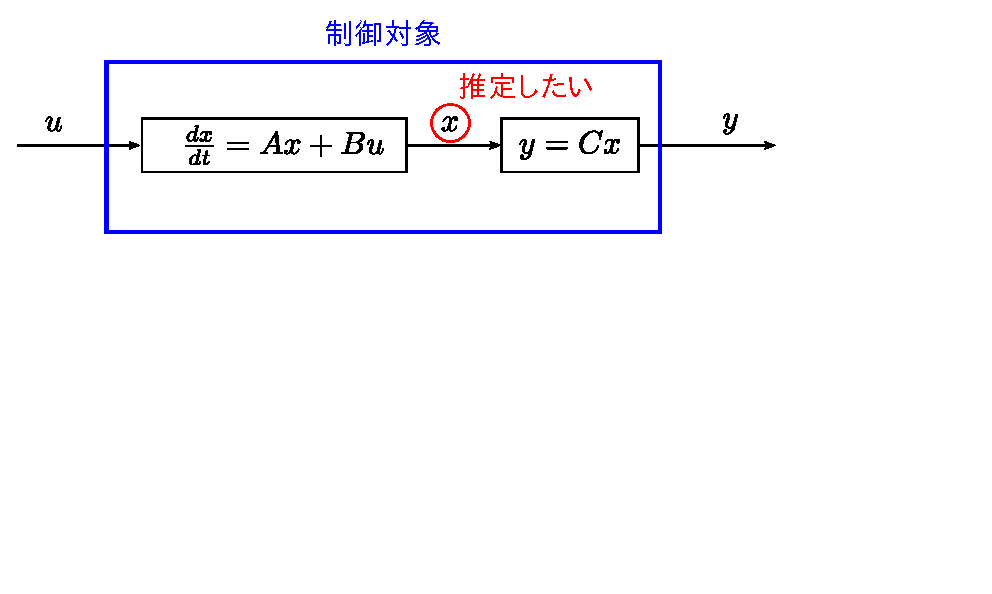
\includegraphics[width=0.7\linewidth]{sfigure/observer2.eps}
  \vspace{-3cm}

  \caption{制御対象}
  \label{fig_obs1}
  \vspace{2cm}

  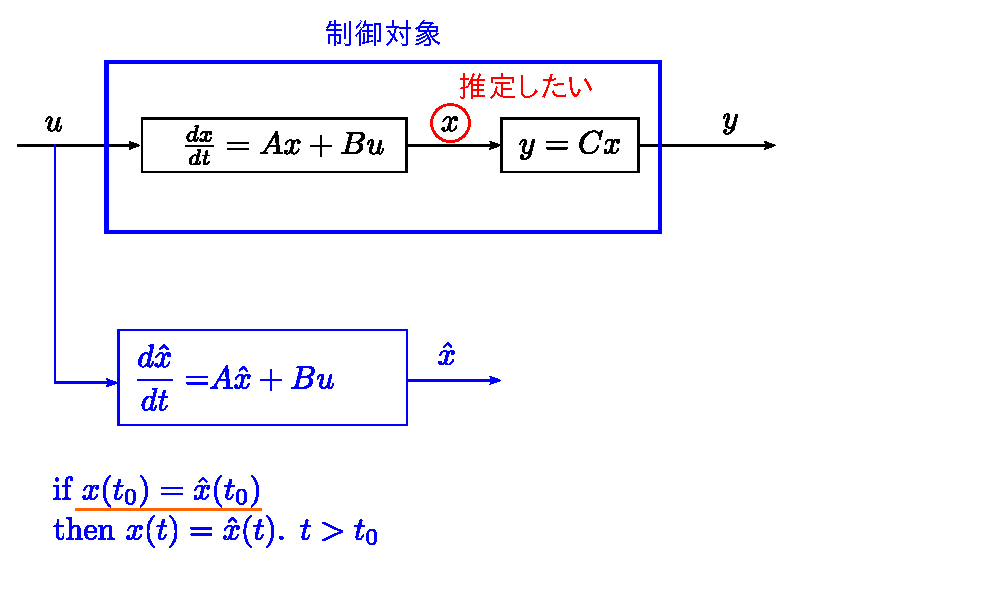
\includegraphics[width=0.7\linewidth]{sfigure/observer3.eps}
  \caption{モデルを用いた状態推定}
  \label{fig_obs2}
  \vspace{2cm}

  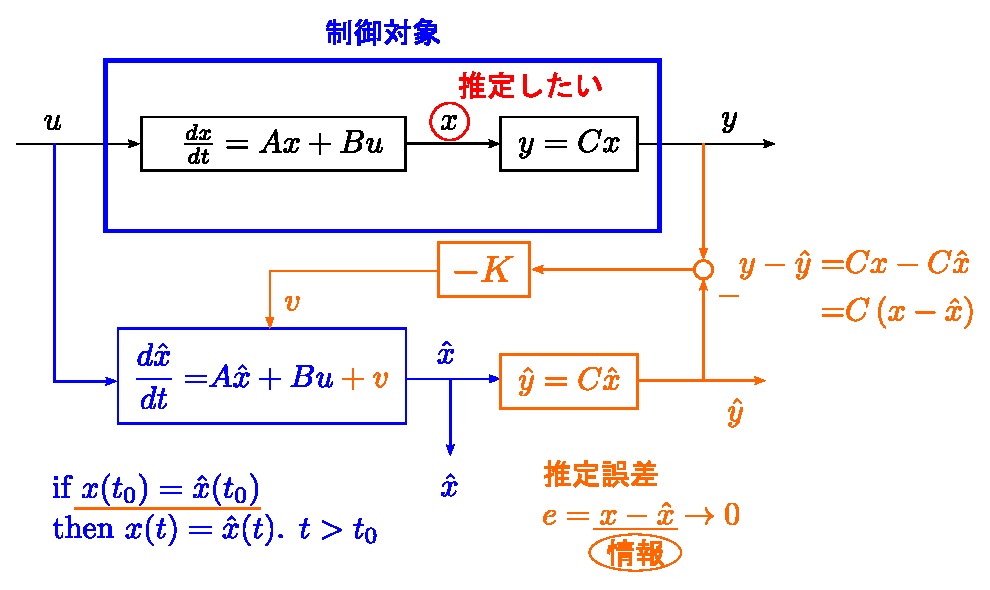
\includegraphics[width=0.7\linewidth]{sfigure/observer5.eps}
  \caption{同一次元オブザーバのブロック線図}
  \label{fig_obs3}
 \end{center}
\end{figure}


いまシステム(\ref{st_proper_state_eq_2})の状態$x$とシステム
(\ref{obs_org})の状態$\hat{x} $の差を
\begin{equation}
 e \defeq x - \hat{x}
\end{equation}
とすれば
\begin{align}
\frac{de}{dt} &= \frac{dx}{dt} - \frac{d \hat{x}}{dt} \nonumber \\
 &= A x + B u - A \hat{x} - B u + K ( y - C \hat{x}) \nonumber \\
 &= A x + B u - A \hat{x} - B u + K ( C x - C \hat{x}) \nonumber \\
 &= A (x - \hat{x}) + K ( C x - C \hat{x}) \nonumber \\
 &= (A + KC) e
\end{align}
となり，$(A+KC)$が安定になるように$K$を選べば，入力や初期値$\hat{x}(0)$に
よらず$e \rightarrow 0$, つまり$\hat{x} \rightarrow x$となることが分かる．このようにシステム
(\ref{obs_org})を用いればシステム(\ref{st_proper_state_eq_2})の状態$x$を
知ることができる．このようなシステムを{\bf オブザーバ(状態観測器)(observer)}と呼ぶ．
$(A + KC)$を安定にする$K$は$(C, A)$が可観測であるときに存在することが知られている．


\subsubsection{簡単なシステムのオブザーバゲインの求め方（例）}

システム
\begin{align}
 \frac{d}{dt}
 \left(
 \begin{array}{c}
  x_1 \\
  x_2
 \end{array}
 \right)
 &=
 \left(
 \begin{array}{cc}
  0 & -1 \\
  1 & 1
 \end{array}
 \right)
 \left(
 \begin{array}{c}
  x_1 \\
  x_2
 \end{array}
 \right) +
 \left(
 \begin{array}{c}
  1 \\
  1
 \end{array}
 \right) u \\
 y &=
 \left(
 \begin{array}{cc}
  0 & 1
 \end{array}
 \right)
 \left(
 \begin{array}{c}
  x_1 \\
  x_2
 \end{array}
 \right)
\end{align}
に対して，同一次元オブザーバ
\begin{equation}
 \frac{d}{dt}
 \left(
 \begin{array}{c}
  \hat{x}_1 \\
  \hat{x}_2
 \end{array}
 \right)
 =
 \left(
 \begin{array}{cc}
  0 & -1 \\
  1 & 1
 \end{array}
 \right)
 \left(
 \begin{array}{c}
  \hat{x}_1 \\
  \hat{x}_2
 \end{array}
 \right) +
 \left(
 \begin{array}{c}
  1 \\
  1
 \end{array}
 \right) u -
 K\left\{y - 
 \left(
 \begin{array}{cc}
  0 & 1
 \end{array}
 \right)
 \left(
 \begin{array}{c}
  \hat{x}_1 \\
  \hat{x}_2
 \end{array}
 \right)\right\}
\end{equation}
の極($(A+KC)$の極)が$-1, -2$となる$K$
\begin{align}
 K&=
 \left( 
 \begin{array}{c}
  k_1 \\
  k_2
 \end{array}
 \right)
\end{align}
を求める．
状態の推定誤差を$e = x - \hat{x}$すると，
\begin{align}
 \frac{de}{dt}
 &= (A+KC) e
 \nonumber \\
 &=
 \left\{
 \left(
 \begin{array}{cc}
  0 & -1 \\
  1 & 1
 \end{array}
 \right)
 + 
 \left( 
 \begin{array}{c}
  k_1 \\
  k_2
 \end{array}
 \right)
 \left(
 \begin{array}{cc}
  0 & 1
 \end{array}
 \right)
 \right\} e
\nonumber \\
 &=
 \left(
 \begin{array}{cc}
  0 & -1 +k_1\\
  1 & 1 + k_2
 \end{array}
 \right)  e
\end{align}
となる．この特性多項式は
\begin{align}
 \det (sI-(A+KC))
 &=\det 
  \left(
  \begin{array}{cc}
   s & 1 -k_1\\
   -1 & s-1 - k_2
  \end{array}
  \right)
 = s^2 + (-k_2 - 1)s + (-k_1 + 1)
\end{align}
である．
一方，極が$-1, -2$となる特性多項式$(s+1)(s+2) = s^2 + 3s + 2$との
係数比較より$k_1 = -1$, $k_2 = -4$となるので，求めるオブザーバのゲイン$K$は
\[
 K = 
 \left(
 \begin{array}{c}
  -1 \\
  -4
 \end{array}
 \right)
\]
と求めることができる．
これを元の同一次元オブザーバに戻すとその状態方程式は
\begin{align}
 \frac{d}{dt}
 \left(
 \begin{array}{c}
  \hat{x}_1 \\
  \hat{x}_2
 \end{array}
 \right)
 =&
 \left(
 \begin{array}{cc}
  0 & -1 \\
  1 & 1
 \end{array}
 \right)
 \left(
 \begin{array}{c}
  \hat{x}_1 \\
  \hat{x}_2
 \end{array}
 \right) +
 \left(
 \begin{array}{c}
  1 \\
  1
 \end{array}
 \right) u -
  \left(
 \begin{array}{c}
  -1 \\
  -4
 \end{array}
 \right)
\left\{y - 
 \left(
 \begin{array}{cc}
  0 & 1
 \end{array}
 \right)
 \left(
 \begin{array}{c}
  \hat{x}_1 \\
  \hat{x}_2
 \end{array}
 \right)\right\} \notag \\
=& 
 \left(
 \begin{array}{cc}
  0 & -2 \\
  1 & -3
 \end{array}
 \right)
 \left(
 \begin{array}{c}
  \hat{x}_1 \\
  \hat{x}_2
 \end{array}
 \right) +
 \left(
 \begin{array}{c}
  1 \\
  1
 \end{array}
 \right) u -
  \left(
 \begin{array}{c}
  -1 \\
  -4
 \end{array}
 \right)
y
\end{align}
となる．

\subsubsection{オブザーバゲインの求め方（状態フィードバックの設計を応用）}


オブザーバのゲイン$K$は状態フィードバックの設計法を応用して次のように求められる．次の状態方程式を考える．
\begin{equation}
 \frac{d \xi}{dt} = A^T \xi + C^T \eta
\label{obs_pole_tmp}
\end{equation}
この状態方程式を安定化させる状態フィードバック
\begin{equation}
 \eta =  K^T \xi
\end{equation}
を求めれば$A^T + C^T K^T$が安定になる．この$K$により$A + K C$も安定となることは正方行列$M$と$M^T$の固有値が等しいことから明らかである．後の双対性の部分で述べるようにオブザーバを設計すべき元のシステム(\ref{st_proper_state_eq_2})(\ref{st_proper_output_eq_2})が可観測である時にシステム(\ref{obs_pole_tmp})は可制御になるから，可観測なシステムはこの方法でオブザーバを設計できることになる．

$M$と$M^T$の固有値が等しいことは以下のように証明できる．行列$M$が
\begin{align}
   T^{-1}MT = \Lambda
\end{align}
と対角化できたとする．この時$\Lambda$の対角要素は$M$の固有値からなっている．ここで$T^{-1}MT$を
転置すると，
\begin{align}
   (T^{-1}MT)^T &=  \Lambda^T = \Lambda
\\
   (T^{-1}MT)^T &= T^T M^T T^{-T} = (T^{-T})^{-1} M^T T^{-T} = \bar{T}^{-1} M^T \bar{T}
   , \ \ \ \bar{T} = T^{-T} 
\end{align}
より
%----------------------footnote
\footnote{
$T^{-T}$は$T^{-T} = (T^{-1})^T$と定義され，$T^{-T} = (T^{-1})^T=(T^T)^{-1}$であることが知られている．
}
%----------------------footnote
\begin{align}
   \bar{T}^{-1} M^T \bar{T} &=  \Lambda
\end{align}
となる．これは$M^{T}$が$\bar{T}$により$\Lambda$に対角化されることを意味している．よって，$\Lambda$の対角要素は$M^{T}$の固有値でもある．つまり，$M$と$M^{T}$
の固有値は等しい．
\subsubsection{例題}

先の例題を考える．
\begin{align}
 \frac{d}{dt}
 \left(
 \begin{array}{c}
  x_1 \\
  x_2
 \end{array}
 \right)
 &=
 \left(
 \begin{array}{cc}
  0 & -1 \\
  1 & 1
 \end{array}
 \right)
 \left(
 \begin{array}{c}
  x_1 \\
  x_2
 \end{array}
 \right) +
 \left(
 \begin{array}{c}
  1 \\
  1
 \end{array}
 \right) u \\
 y &=
 \left(
 \begin{array}{cc}
  0 & 1
 \end{array}
 \right)
 \left(
 \begin{array}{c}
  x_1 \\
  x_2
 \end{array}
 \right)
\end{align}
このシステムのオブザーバを設計するときに，$(A+KC)$の極（オブザーバの極）が$-1,-2$と
なるように$K$を定めるため，次のシステムの状態フィードバック（極配置）問題を考える．
\begin{align}
 \frac{d\xi}{dt} &= A^T \xi + C^T \eta \nonumber \\
 &=
 \left(
 \begin{array}{cc}
  0 & 1 \\
  -1 & 1
 \end{array}
 \right) \xi +
 \left(
 \begin{array}{c}
  0 \\
  1
 \end{array}
 \right) \eta
\end{align}
いま$\eta = K^T \xi = (\begin{array}{cc}k_1 & k_2\end{array})\xi$とする
と，
\begin{equation}
 \frac{d\xi}{dt} =
 \left(
 \begin{array}{cc}
  0 & 1 \\
  -1+k_1 & 1 + k_2
 \end{array}
 \right) \xi
\end{equation}
となり，この特性多項式は$s^2 + (-k_2 - 1)s + (-k_1 + 1)$である．
一方，極が$-1, -2$となる特性多項式$(s+1)(s+2) = s^2 + 3s + 2$との
係数比較より$k_1 = -1$, $k_2 = -4$となるので，求めるオブザーバのゲイン$K$は
\[
 K = 
 \left(
 \begin{array}{c}
  -1 \\
  -4
 \end{array}
 \right)
\]
と求めることができる．これは先の結果と一致する．
\\

\noindent
{\bf ＜演習＞オブザーバ} \nopagebreak

次のシステムに対して，オブザーバを設計せよ．ただし，オブザーバの極は$-1,-2$とせよ．
\begin{align*}
	\frac{d}{dt}
	\left (
	\begin{array}{c}
	 x_1 \\ x_2 
	\end{array}
	\right )
	& = 
	\left (
	\begin{array}{cc}
	 0 & 2 \\
	 1 & -1
	\end{array}
	\right )
	\left (
	\begin{array}{c}
	 x_1 \\ x_2 
	\end{array}
	\right )
	+
	\left (
	\begin{array}{c}
	 1 \\ 1 
	\end{array}
	\right )
	u
\\
	y&=
	\left ( \begin{array}{cc}
		0 & 2 
	\end{array} \right )
	\left (	\begin{array}{c}
		x_1 \\ x_2 
	\end{array} \right )
\end{align*}

%---------------------------------------------------------------------------
\subsection{オブザーバによる状態フィードバック系の安定性}
%---------------------------------------------------------------------------
システム
\begin{align}
 \frac{dx}{dt} &= A x + B u \\
 y             &= C x
\end{align}
を安定化する状態フィードバックが
\begin{equation}
 u = F x
\end{equation}
で与えられているとする．
また，同一次元オブザーバが
\begin{equation}
 \frac{d \hat{x}}{dt} = A \hat{x} + B u - K (y - C \hat{x})
  \label{eq:obs}
\end{equation}
で与えられているとき，状態$x$を推定値$\hat{x}$で置き換えたフィードバック
則
\begin{equation}
 u = F \hat{x}
\end{equation}
を用いたときのシステムの安定性について考える．
ただし，$A + BF$が安定となるように$F$は選ばれ，
$A + KC$が安定となるように$K$が選ばれていると仮定する．
Fig.\ref{fig_obs_feedback}には
オブザーバを用いたフィードバック系の構成を示している．
\begin{figure}[htbp]
 \begin{center}
  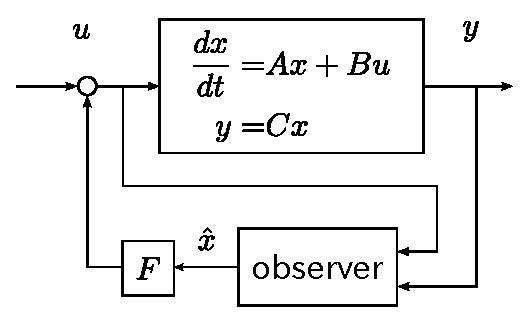
\includegraphics[width=0.4\linewidth]{sfigure/observer_simple.eps} % scale = 100%
  \caption{オブザーバを用いたフィードバック系}
  \label{fig_obs_feedback}
 \end{center}
\end{figure}

結論から言えば，このオブザーバを用いた閉ループ系の極は状態フィードバックを設計したときの極とオブザーバの極と一致するため，両者を安定に設計すれば閉ループ系が必ず安定となる．これは次のように証明できる．


まず，システムとオブザーバを合わせたシステム(併合系)は
\begin{equation}
 \frac{d}{dt}
  \left(\begin{array}{c}
         x \\
	 \hat{x}
	\end{array}\right)
  =
  \left(\begin{array}{cc}
         A & 0 \\
	 -KC & A+KC
	\end{array}\right)
  \left(\begin{array}{c}
         x \\
	 \hat{x}
	\end{array}\right)
  +
  \left(\begin{array}{c}
         B \\
	 B
	\end{array}\right)
  u
  \label{eq:hoge}
\end{equation}
となる．
ここで，次のような座標変換を考える．
\begin{equation}
 \left(\begin{array}{c}
         x \\
	 \hat{x}
       \end{array}\right)
 =
 \left(\begin{array}{cc}
        I & 0 \\
	I & -I
       \end{array}\right)
 \left(\begin{array}{c}
         x \\
	 x - \hat{x}
       \end{array}\right)
 \defeq T
 \left(\begin{array}{c}
         x \\
	 e
       \end{array}\right)
\end{equation}
\ref{sec:zahyohenkan}節の座標変換に従うと，(\ref{eq:hoge})は次のように書き直せる．
\begin{align}
 \frac{d}{dt}
  \left(\begin{array}{c}
         x \\
	 e
	\end{array}\right)
  &=
  T^{-1}
  \left(\begin{array}{cc}
         A & 0 \\
	 -KC & A+KC
	\end{array}\right)
  T
  \left(\begin{array}{c}
         x \\
	 e
	\end{array}\right)
  +
  T^{-1}
  \left(\begin{array}{c}
         B \\
	 B
	\end{array}\right)
  u
\nonumber \\
  &=
 \left(\begin{array}{cc}
        I & 0 \\
	I & -I
       \end{array}\right)
  \left(\begin{array}{cc}
         A & 0 \\
	 -KC & A+KC
	\end{array}\right)
 \left(\begin{array}{cc}
        I & 0 \\
	I & -I
       \end{array}\right)
  \left(\begin{array}{c}
         x \\
	 e
	\end{array}\right)
  +
 \left(\begin{array}{cc}
        I & 0 \\
	I & -I
       \end{array}\right)
  \left(\begin{array}{c}
         B \\
	 B
	\end{array}\right)
  u
\nonumber \\
  &=
  \left(\begin{array}{cc}
         A & 0 \\
	 0 & A+KC
	\end{array}\right)
  \left(\begin{array}{c}
         x \\
	 e
	\end{array}\right)
  +
  \left(\begin{array}{c}
         B \\
	 0
	\end{array}\right)
  u
\end{align}
このシステムではオブザーバの推定誤差にあたる$e=x-\hat{x}$が不可制御となっている．これは，オブザーバ誤差$e$が入力$u$によらず$0$に収束することから，当然なことである．

さて，この状態方程式に状態$x$の代わりにオブザーバの状態$\hat{x}$で置き換えたフィードバック
\begin{align}
 u &= F \hat{x}
\nonumber \\
   &= F \{x - (x-\hat{x})\}
\nonumber \\
   &= F (x - e) 
    = \left( \begin{array}{cc} F & -F \end{array} \right)
      \left( \begin{array}{c}
               x \\
               e 
             \end{array} \right)
\end{align}
を代入すれば，状態方程式は次のようになる．
\begin{align}
 \frac{d}{dt}
  \left(\begin{array}{c}
         x \\
	 e
	\end{array}\right)
  &=
  \left(\begin{array}{cc}
         A & 0 \\
	 0 & A+KC
	\end{array}\right)
  \left(\begin{array}{c}
         x \\
	 e
	\end{array}\right)
  +
  \left(\begin{array}{c}
         B \\
	 0
	\end{array}\right)
  \left( \begin{array}{cc} F & -F \end{array} \right)
  \left( \begin{array}{c}
               x \\
               e 
         \end{array} \right)
\nonumber \\
 &=
 \left(\begin{array}{cc}
        A + BF & -BF \\
	0 & A + KC
       \end{array}\right)
 \left(\begin{array}{c}
         x \\
	 e
       \end{array}\right)
\end{align}
となる．このシステムの極は特性多項式
\begin{equation}
 \det\left\{s I - \left(\begin{array}{cc}
		         A + BF & -BF \\
			 0 & A + KC
			\end{array}\right)\right\}
 =
 \det\left(\begin{array}{cc}
            sI - (A + BF) & BF \\
	    0 & sI - (A + KC) \\
	   \end{array}\right)
\end{equation}
の根となる．ブロック3角行列の行列式の性質より，これは
\begin{equation}
 = \det(sI - (A + BF))\det(sI - (A + KC))
\end{equation}
となるから，同一次元オブザーバを用いたフィードバック系の極が，
フィードバックによるシステムの極($A + BF$の固有値)と同一次元オブザーバの極
($A + KC$の固有値)と一致することが分かる．
つまり{\bf 状態フィードバックとオブザーバを個別に設計しても全体の安定性が保証される}ことが分かる．





%---------------------------------------------------------------------------
\section{カルマンフィルタ}
%---------------------------------------------------------------------------

前節では状態$x$を推定するためにオブザーバを考えた．オブザーバ＋状態フィードバックの併合系の極はオブザーバの極と状態フィードバックの極に一致するので，システムの安定化を図るためには安定なオブザーバを設計するだけでよいことになる．しかし，実際にはどのようなことを考慮に入れてオブザーバを設計する必要があるのだろうか，ここではシステムに外乱（雑音）が入る場合の最適な状態推定（カルマンフィルタ）について考える．

\subsubsection{確率外乱の入るシステム}

ここでは状態方程式と出力方程式に確率的な外乱$v,w$の入る次のシステムを考える．
\begin{align}
 \frac{dx}{dt} &= A x(t) + B u(t) +  v \label{state_eq_dis} \\
 y(t) &= C x(t) + w \label{output_eq_dis}
\end{align}
ここで状態，入力，出力はそれぞれ$x \in {\mathbb R}^n$, $ u \in {\mathbb R}^m $, $ y \in {\mathbb
R}^p $である．また，$v \in {\mathbb R}^n$, $w \in {\mathbb R}^p$はそれぞれ{\bf システム雑音(system noise)}, {\bf 観測雑音(observation noise)}であり，独立な正規分布に従う白色雑音過程と仮定する．つまり，$E\{ a \} = \bar{a} $を$a$の期待値，$\mbox{cov}(a,b) = E \{ (a-\bar{a})(b-\bar{b})^T \}$を$a$と$b$の共分散行列とするとき，$v$と$w$の統計的性質が
\begin{align}
     E \{ v(t) \} = \bar{v} = 0, & \ \ \ \mbox{cov}\{ v(t), v(\tau)\} = V \delta(t-\tau)
\\
     E \{ w(t) \} = \bar{w} = 0, & \ \ \ \mbox{cov}\{ w(t), w(\tau)\} = W \delta(t-\tau)
\\
                       & \ \ \ \mbox{cov} \{v(t), w(\tau) \} =0  
\end{align}
と表されるとする．ただし，
\begin{align}
	\delta(a)
	&= \left \{
		\begin{array}{ll}
			1 & (a =    0) \\
			0 & (a \neq 0)
		\end{array}
	   \right .
\end{align}
つまり，$v(t)$の値は時刻が違う$v(\tau)$と無相関であるが，同じ時刻の$v(t)$の値とは$V$で特徴付けられる共分散を持つことを意味している．$w(t)$についても同様である．また，$v(t)$と$w(\tau)$の共分散行列が時刻$t,\tau$に無関係に$0$となるということは$v(t)$と$w(\tau)$が無相関であることを意味している．


\subsubsection{カルマンフィルタ}

確率雑音の入るシステムで状態$x$を最適に推定する問題を考える．評価関数として状態$x(t)$の推定値$\hat{x}(t)$の推定誤差$e(t) = x(t) - \hat{x}(t)$の二乗を考える．
\begin{align}
     J_o = E\{ \vert e(t) \vert^2 \} = E\{ \vert x(t) - \hat{x}(t) \vert^2 \}
\end{align}
$(C,A)$可観測の場合，この評価関数を最小とする状態の推定値$\hat{x}(t)$は以下のオブザーバで得られることがわかっている．これを{\bf カルマンフィルタ(Kalman filter)}と呼ぶ．
\begin{align}
 \frac{d \hat{x}}{dt} =& A \hat{x} + B u - K (y - C \hat{x})
\\
 & K = -\Sigma C^T W^{-1}
\end{align}
ただし，$\Sigma$は以下のリカッチ方程式の正定解である．
\begin{align}
 & A \Sigma + \Sigma A^T +  V - \Sigma C^T W^{-1} C \Sigma = 0
\label{riccati_kalman}
\end{align}
このリカッチ方程式は最適制御のリカッチ方程式において
\begin{align}
   \Sigma \leftrightarrow P,   \ \ 
   A^T    \leftrightarrow A, \ \ 
   C^T    \leftrightarrow B, \ \ 
   W      \leftrightarrow R, \ \ 
   V      \leftrightarrow Q, \ \ 
   K^T    \leftrightarrow F 
\end{align}
としたものとなっている．

カルマンフィルタを実際に設計する際には外乱$v$, $w$の統計的性質はわかってはいないので，$V$, $W$は設計のためのパラメータと考えることができる．いま
\begin{align}
	V =    \left(
			\begin{array}{cccc}
				\alpha_1 & & & \\
				& \alpha_2 & & \\
				& & \ddots & \\
				& & & \alpha_n \\
			\end{array}
		\right)
\hspace{1cm}
	W =    \left(
			\begin{array}{cccc}
				\beta_1 & & & \\
				& \beta_2 & & \\
				& & \ddots & \\
				& & & \beta_p \\
			\end{array}
		\right)
\end{align}
とすると，$\alpha_1$が大きいということは定義より$v_1$(外乱$v$の第1成分)が大きいということ，つまり，$x_1$に対する外乱が大きいということを意味する．このとき，最適推定をするためには外乱により変動する$x_1$をいち速く推定しないといけないこととなる．そこで，例えば$x_1$に対する推定が遅いようならば$\alpha_1$を大きくしてカルマンフィルタを再設計することにより，$x_1$の推定値の収束を速めることが期待される．一方，$\beta_1$が大きいということは$y_1$の測定外乱($w$の第1成分である$w_1$)が大きいことを示している．$\beta_1$が大きい場合に最適推定するためには$y_1$の情報をあまり信用しないで推定することが必要となる．そこで，例えば$y_1$に外乱が大きく作用しているため推定値が大きく変動するようならば，$\beta_1$を大きくしてカルマンフィルタを再設計することにより$y_1$を信用しないカルマンフィルタが構成されることが期待できる．もちろん，この場合は推定値の収束は遅くなる．

\subsubsection{カルマンフィルタの補足}

実は先のカルマンフィルタの記述は，オブザーバとしてのカルマンフィルタを設計するには十分であるが，理論的には厳密ではない．数学としてカルマンフィルタを厳密に記述すると以下のようになる．

まず，状態の初期値$x(0)$は不明であるが，平均が$\bar{x}_0$, 分散が$\Sigma_0$である正規分布に従っていると仮定する．つまり，
\begin{align}
     E\{x(0) \} = \bar{x}_0, \ \ \ \mbox{cov} \{ x(0), x(0) \} = \Sigma_0
\end{align}
とする．このとき推定誤差の二乗期待値である評価関数$J_0$を最小にする状態$x(t)$の推定値$\hat{x}(t)$は以下で与えられる．
\begin{align}
 \frac{d \hat{x}}{dt} =& A \hat{x} + B u - K(t) (y - C \hat{x})
\\
 & K(t) = - \Sigma(t) C^T W^{-1}
\\
 & \hat{x}(0) = \bar{x}_0
\\
 - \frac{d \Sigma}{dt} = & A \Sigma(t) + \Sigma(t) A^T +  V ^T - \Sigma(t) C^T W^{-1} C \Sigma(t)
\label{riccati_kalman_dif}
\\
 & \Sigma(0) = \Sigma_0
\end{align}
ここでオブザーバの初期値が$\hat{x}(0)=\bar{x}_0$であること，また，リカッチ方程式(\ref{riccati_kalman})がリカッチ微分方程式(\ref{riccati_kalman_dif})になっていることに注意する．
さらに
\begin{align}
     \Sigma(t) &= \mbox{cov} \{ e(t), e(t) \} = \mbox{cov} \{ x(t)-\hat{x}(t),  x(t)-\hat{x}(t)\} 
\nonumber\\
     &= E \{ [x(t)-\hat{x}(t)][x(t)-\hat{x}(t)]^T \}
\end{align}
となっていることが知られている．


$(C,A)$可観測の場合，このリカッチ微分方程式(\ref{riccati_kalman_dif})の解$\Sigma(t)$が$t \rightarrow \infty$でリカッチ方程式(\ref{riccati_kalman})の半正定解$\Sigma$に収束することが示されている．


\subsubsection{分離定理}

確率外乱の入るシステム(\ref{state_eq_dis})(\ref{output_eq_dis})に対する最適制御も研究されている．

次の評価関数を考える($E$は期待値)．
\begin{align}
  J=\lim_{t_f \rightarrow \infty} \frac{1}{t_f} E \left\{\int_0^{t_f} x^T Q x + u^T R u \ dt \right\}
\end{align}
この評価関数を最小とする状態フィードバックが\ref{sec_opt}の最適制御と一致することが証明されている．また，この状態フィードバックの状態$x$をカルマンフィルタの推定値$\hat{x}$で置き換えたものが，評価関数を最小とする出力フィードバックであることも証明されている．

このように，確率外乱の入るシステムにおいては最適制御とカルマンフィルタは単にフィードバック系の安定化を保証するのみならず，制御の最適性まで保証する．このように最適制御と最適推定（カルマンフィルタ）の組み合わせコントローラが最適な出力フィードバックとなることを保証することは分離定理と呼ばれている．


\section{双対性}
%---------------------------------------------------------------------------

システムの可制御性と可観測性，状態フィードバックの設計と同一次元オブザーバの設計，最適制御とカルマンフィルタには{\bf 双対性(duality)}と呼ばれる性質がある．

元のシステム(\ref{state_eq})(\ref{output_eq})に対して次のシステムを{\bf 双対システム(dual system)}と呼ぶことがある．
\begin{align}
 \frac{d \tilde{x}}{dt} &= A^T \tilde{x}(t) + C^T \tilde{u}(t) \label{state_eq_dual} \\
 \tilde{y}(t) &= B^T \tilde{x}(t) + D^T \tilde{u}(t) \label{output_eq_dual}
\end{align}
このシステムの伝達関数$\tilde{G}(s)$は
\begin{align}
	\tilde{G}(s) &= B^T (sI-A^T)^{-1} C^T + D^T = \{C(sI-A)^{-1}B + D\}^T = G(s)^T
\end{align}
となり，元のシステム(\ref{state_eq})(\ref{output_eq})の伝達関数$G(s)$を転置したものになっている．

元のシステム(\ref{state_eq})(\ref{output_eq})の可観測性を確認するための行列
\begin{align}
 N^T =
  \left( \begin{array}{c}
         C        \\
	 C A      \\
	 C A^2    \\
	 \vdots   \\
	 C A^{n-1}
  \end{array} \right)
\nonumber
\end{align}
は双対システム(\ref{state_eq_dual})(\ref{output_eq_dual})の可制御性を確認するための行列
\begin{align}
     \tilde{V} = \{C^T, A^T C^T, (A^T)^2 C^T , \cdots (A^T)^{n-1} C^T　\}
\nonumber
\end{align}
と
\begin{align}
  N = \tilde{V}
\end{align}
の関係にある．

また，元のシステム(\ref{state_eq})(\ref{output_eq})に対して同一次元オブザーバを設計するためには$(A+KC)$が安定となるようにオブザーバゲイン$K$を設計する必要があるが，双対システム(\ref{state_eq_dual})(\ref{output_eq_dual})を安定化するフィードバック$\tilde{u} =  K^T \tilde{x}$は
$(A^T + C^T K^T)$を安定化する．つまり，$(A + K C) = (A^T + C^T K^T)^T$を安定化する．これは双対システムを安定化するフィードバック$\tilde{u} =  K^T \tilde{x}$を設計することによりオブザーバゲインを設計することが可能となることを示している．このとき極配置問題を解いて双対システムを安定化するフィードバックを設計すれば元のシステムに対する極配置オブザーバを設計することと同値となる．
また，先に述べたように双対システム(\ref{state_eq_dual})(\ref{output_eq_dual})に対する最適制御の設計問題（リカッチ方程式）は元のシステム(\ref{state_eq})(\ref{output_eq})に対するカルマンフィルターゲイン$K$の設計問題（リカッチ方程式）と同値となる．

\begin{center}
\begin{tabular}{ccc}
	元のシステム				&					&	双対システム	\\
	可制御性					& $\Leftrightarrow$ &	可観測性 \\
	可観測性					& $\Leftrightarrow$ &	可制御性 \\
	状態フィードバック（極配置）& $\Leftrightarrow$ &	オブザーバ（極配置） \\
	オブザーバ（極配置）		& $\Leftrightarrow$ &	状態フィードバック（極配置） \\
	最適制御					& $\Leftrightarrow$ &	カルマンフィルタ \\
	カルマンフィルタ			& $\Leftrightarrow$ &	最適制御 \\
\end{tabular}
\end{center}
\ \\

\noindent
{\bf 双対性に対する補足}

作用素論的に厳密にいえば，次のシステムが双対システムである．
\begin{align}
 \frac{d \tilde{x}}{dt} &= -A^T \tilde{x}(t) - C^T \tilde{u}(t) \label{state_eq_dual_2} \\
 \tilde{y}(t) &= B^T \tilde{x}(t) + D^T \tilde{u}(t) \label{output_eq_dual_2}
\end{align}
このシステムの伝達関数$\tilde{G}(s)$は
\begin{align}
	\tilde{G}(s) &= - B^T (sI+A^T)^{-1} C^T + D^T=  B^T (-sI-A^T)^{-1} C^T + D^T 
\nonumber \\
	&= \{C(-sI-A)^{-1}B + D\}^T = G(-s)^T
\end{align}
となり，元のシステム(\ref{state_eq})(\ref{output_eq})の伝達関数$G(s)$を転置し，$s$を$-s$に置き換えたものである．

しかし，ここでは可制御性・可観測性，状態フィードバック・オブザーバ，最適制御・カルマンフィルタに関する形式がわかりやすいように先のシステムを双対システムとして考えた．

